%% Submissions for peer-review must enable line-numbering 
% * <markusgwalsh@gmail.com> 2018-03-06T15:27:58.924Z:
%
% ^.
%% using the lineno option in the \documentclass command.
%%
%% Preprints and camera-ready submissions do not need 
%% line numbers, and should have this option removed.
%%
%% Please note that the line numbering option requires
%% version 1.1 or newer of the wlpeerj.cls file, and
%% the corresponding author info requires v1.2

\documentclass[fleqn,10pt,lineno]{wlpeerj} % for journal submissions
% \documentclass[fleqn,10pt]{wlpeerj} % for preprint submissions
%\usepackage[natbibapa]{apacite} % print full list of authors names in the biblio
\usepackage{nameref,hyperref}
\usepackage{setspace}
\usepackage{amsmath} %% break long equations
\usepackage[normalem]{ulem} % use normalem to protect \emph
\useunder{\uline}{\ul}{}
\usepackage[binary-units=true]{siunitx}  %% SI Units
\usepackage{longtable}
\usepackage{url}
\usepackage[noae]{Sweave}
\hypersetup{colorlinks=true, linkcolor=blue, citecolor=red, bookmarksnumbered=true,
        urlcolor=blue, bookmarksopen=true, pdfview=FitH, pdfstartview=FitH,
        pdftitle={Mapping Potential Natural Vegetation},
        pdfauthor={Hengl et al.}} %%
%% fix the font size and encoding for url's etc:
\newcommand\hl{\noindent\bgroup\markoverwith{\textcolor{yellow}{\rule[-.5ex]{2pt}{2.5ex}}}\ULon} %% highlight some lines
%% fix the font size and encoding for url's etc:
\renewcommand{\ttdefault}{cmtt}
\renewcommand{\sfdefault}{cmss}

\title{Global Mapping of Potential Natural Vegetation: An Assessment of Machine Learning Algorithms for Estimating Land Potential}
\author[1]{Tomislav Hengl}
\author[2,3]{Markus G. Walsh}
\author[4]{Jonathan Sanderman}
\author[1]{Ichsani Wheeler}
\author[5]{Sandy P. Harrison}
\author[6]{Iain C. Prentice}
\affil[1]{Envirometrix Ltd., Wageningen, the Netherlands}
\affil[2]{The Earth Institute, Columbia University, USA}
\affil[3]{Selian Agricultural Research Inst., Arusha, Tanzania}
\affil[4]{Woods Hole Research Center, MA USA}
\affil[5]{School of Archeology, Geography and Environmental Science, University of Reading, UK}
\affil[6]{AXA Chair of Biosphere and Climate Impacts, Grand Challenges in Ecosystem and the Environment, Department of Life Sciences and Grantham Institute --- Climate Change and the Environment, Imperial College London, UK}
\corrauthor[1]{Tomislav Hengl}{tom.hengl@envirometrix.net}
%\keywords{natural vegetation, random forest, historic vegetation, global, biome}

\begin{abstract}
Potential Natural Vegetation (PNV) is the vegetation cover in equilibrium with climate, that would exist at a given location if not impacted by human activities. PNV is useful for raising public awareness about land degradation and for estimating land potential. This paper presents results of assessing Machine Learning Algorithms (MLA) --- neural networks (\textsf{nnet} package), random forest (\textsf{ranger}), gradient boosting (\textsf{gmb}), K-nearest neighborhood (\textsf{class}) and \textsf{cubist} --- for operational mapping of PNV. Three case studies were considered: (1) global distribution of biomes based on the BIOME 6000 data set (8057 modern pollen-based site reconstructions), (2) distribution of forest tree taxa in Europe based on detailed occurrence records (1,546,435 ground observations), and (3) global monthly Fraction of Absorbed Photosynthetically Active Radiation (FAPAR) values (30,301 randomly-sampled points). A stack of 160 global maps representing biophysical conditions over land, including atmospheric, climatic, relief and lithologic variables, were used as explanatory variables. Overall, random forest models gave the best performance. The highest accuracy for predicting BIOME 6000 classes (20) was estimated to be between \SI{33}{\percent} (with spatial Cross Validation) and \SI{68}{\percent} (simple random subsetting), with the most important predictors being total annual precipitation, monthly temperatures and bioclimatic layers. Predicting forest tree species (73) resulted in mapping accuracy of \SI{25}{\percent}, with the most important predictors being monthly cloud fraction, mean annual and monthly temperatures and elevation. Regression models for FAPAR (monthly images) gave an R-square of \SI{90}{\percent} with the most important predictors being total annual precipitation, monthly cloud fraction, CHELSA bioclimatic layers and month of the year, respectively. Further developments of PNV mapping could include using all GBIF records to map the global distribution of plant species at different taxonomic levels. This methodology could also be extended to dynamic modeling of PNV, so that future climate scenarios can be incorporated. Global maps of biomes, FAPAR and tree species at \SI{1}{\kilo\metre} spatial resolution are available for download via \url{http://dx.doi.org/10.7910/DVN/QQHCIK}.
\end{abstract}

\linespread{1.4}
\begin{document}

%\flushbottom
\maketitle\thispagestyle{empty}
\hl{Submitted to PeerJ on 26th of March 2018; 1st revision on 8th of July 2018;}

\section*{Introduction}

Potential Natural Vegetation (PNV) is the \emph{``vegetation cover in equilibrium with climate, that would exist at a given location non-impacted by human activities''} \citep{levavasseur2012statistical,OstbyeHemsing2012}. It is a hypothetical vegetation state assuming natural (undisturbed) physical conditions, a reference status of vegetation assuming no degradation and/or no unusual ecological disturbances. PNV is especially useful for raising public awareness about land degradation \citep{weisman2008world} and for estimating land potential \citep{herrick2013global}. For example, \citet{omernik1987ecoregions} details PNV maps for USA; \citet{bohn2007map} provides maps for EU; \citet{carnahan1989australia} for Australia; \citet{marinova2018pollen} maps PNV for the Eastern Mediterranean--Black Sea--Caspian-Corridor; and maps of PNV for Latin America are available in \citet{marchant2009pollen}. Regarding specific tree species, \citet{san2016european} provide habitat suitability maps for the main forest tree species in Europe, based on environmental variables, especially bioclimatic variables such as average temperature of the coldest month, precipitation of the driest month and similar. \citet{Potapov2011} generated a global map of potential forest cover at \SI{1}{\kilo\metre} resolution (publicly available from \url{http://globalforestwatch.org/map/}). \citet{erb2017unexpectedly} produced a global map of potential biomass stocks by reversing the current managed land use systems to natural vegetation. \citet{levavasseur2012statistical} and \citet{tian2016terrestrial} predict global PNV classes using environmental covariates such as climatic images and landform parameters. \citet{Griscom11645} recently produced a global reforestation map at \SI{1}{\kilo\metre} resolution.\par 

A common limitation of existing maps is their coarse spatial resolution (about \SI{25}{\kilo\metre}) limiting the use of these maps for operational planning (e.g.\@ \citet{marchant2009pollen,levavasseur2012statistical} and \citet{tian2016terrestrial}). In addition, comparisons of multiple overlapping sources of PNV maps shows that they rarely agree with one another since they do not share the same mapping criteria and, traditionally, emphasize regionally-specific botanical groupings rather than functional classifications. Limitations of maps based on field surveys of PNV (e.g., \citet{bohn2007map}) arise from assumptions about controls on vegetation distribution based on extrapolation from a limited number of field surveys. \par

Here we provide an update of comparable global PNV maps produced by \citet{Potapov2011,levavasseur2012statistical,tian2016terrestrial} and \citet{erb2017unexpectedly}. We explore the possibility of increasing the mapping accuracy using up-to-date maps of climate, atmosphere dynamics, landform and lithology, and state-of-the-art machine learning methods. Our final aim is to produce PNV maps that are more detailed, richer in information, based on objective reproducible methods; and potentially more usable for global modeling and awareness raising projects. We focus on improving the spatial detail, thematic accuracy and reproducibility of maps, at the cost of increasing the total computing load. We also consider automation of the prediction process so that the maps can be rapidly updated as new ground truth data is obtained. Our modeling follows three phases: 

\begin{enumerate}\renewcommand{\labelenumi}{(\alph{enumi})}
\item model selection: we compare possible models of interest for PNV mapping and choose the optimal spatial prediction framework based on the cross-validation results,
\item model assessment: we assess the uncertainty of predictions per vegetation class and try to determine objectively the limitations of the mapping products for wider uses, and
\item prediction: we use the best performing models to produce spatial predictions, then visually assess maps and if necessary repeat steps a--c.
\end{enumerate}

\section*{Methods and materials}

\subsection*{Theory}

PNV is the hypothetical vegetation cover that would be present if the vegetation were in equilibrium with environmental controls, including climatic factors and disturbance, and not subject to human management. When considering PNV, one needs to distinguish between potential \emph{``natural'} and potential \emph{``managed''} vegetation, and \emph{``actual''} natural and \emph{``actual''} managed vegetation (Fig.\@~\ref{Fig_concepts_PNV}a). Vegetation is in general a dynamic feature. Also PNV changes as the climatic conditions change. For example, with the future global warming and changes in our climate, PNV might be significantly different than pre-industrial revolution. Therefore it is important to reference PNV  to the time period of interest, so that historic PNV and current or future PNV maps can be produced (Fig.\@~\ref{Fig_concepts_PNV}b).\par

\begin{figure}[!hbt]
\centering
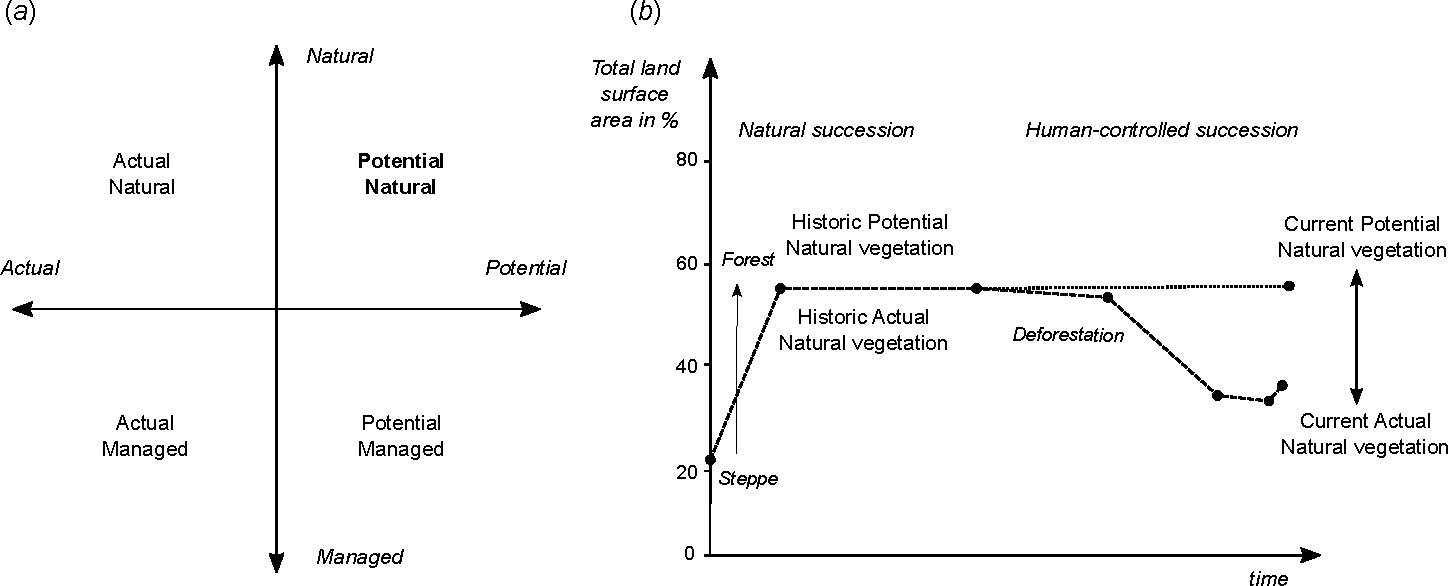
\includegraphics[width=\linewidth]{Fig_1.pdf}
\caption{Schematic explanation of differences between (a) potential and actual natural/managed vegetation, and (b) current and historic vegetation in the context of global land area.}
\label{Fig_concepts_PNV}
\end{figure}

In addition to the differentiation between the potential and actual natural vegetation, there are also three sub-types of the PNV that need to be considered:

\begin{enumerate}
\item PNV model A: based on the autochthonous or native vegetation and living species only.
\item PNV model B: based on the autochthonous or native vegetation that includes also extinct species.
\item PNV model C: PNV based on any vegetation whether native or introduced or extinct.
\end{enumerate}

Derivation of maps of PNV model A could be of interest to e.g.\@ nature conservationists; PNV model C could be of more interest to e.g.\@ forestry and agroforestry organizations as it provides an objective basis for introducing non-native species to a new area.\par 

Conveniently, locations that have not been subject to human disturbance/management can provide relevant information about vegetation cover in historic times, which can serve as a guide to PNV. A major limitation of modeling PNV is that we unfortunately do not have equally detailed information about the status of vegetation and environment across historic periods. For instance, about half of the Earth's mature tropical forests have disappeared in the last 150 years and original habitats have been reduced to \SI{10}{\percent} \citep{hansen2013high}. Given that climates have changed and few areas are truly human impact \emph{``free''}, even undisturbed historic vegetation only represents one possible expression of PNV for a given set of climate conditions at a specific time. \par

Regardless of the hypothetical nature of PNV, the concept (both as a classification and as a regression type problem) is still a helpful yardstick against which land cover change can be quantitatively measured and land restoration designs can be planned. \citet{erb2017unexpectedly} have estimated that almost half of the standing global vegetation biomass carbon stocks has been lost, almost equally due to land cover change (e.g.\@ tree cover to cropland) and management effects within land cover types (e.g.\@ croplands managed at lower biomass carbon stocks than tree covered areas). PNV maps can thus help quantify such differences, both deficit and surplus, in biomass stocks caused by the current land management system more objectively and served as an input to the redesign of land management systems. \par

\subsection*{PNV mapping and species distribution modeling}

In principle, PNV mapping is a special case of species distribution modeling \citep{elith2009species,OstbyeHemsing2012,hijmans2016species}: at the core of PNV mapping is statistical modeling of the relationship between species (or natural associations of species or communities) and a list of predictors i.e.\@ biotic and abiotic site factors \citep{elith2009species}. The difference between mapping actual distribution of species and PNV mapping is that PNV involves extrapolating the model to the whole land mask, assuming a hypothetical distribution under a specific set of undisturbed bioclimatic and/or biophysical conditions:

\begin{equation}\label{E:general}
\Pr(Y) = f \left( \mathrm{Relief}, \mathrm{BioClimate}, \mathrm{Lithology} \right)
\end{equation}

\noindent where $Y$ is the target variable, which could be vegetation types or plant species with a finite number of states $Y \in \{1,2,\ldots,k\}$ and/or vegetation properties. PNV mapping can be considered as a \emph{classification-type} or \emph{regression-type} problem depending on whether we map factors such as vegetation types or continuous vegetation properties such as biomass or leaf area index. \par 

The primary assumptions we make when applying a PNV model to the training data are:

\begin{enumerate}
\item The ecological gradients captured in training data reflect only natural ecological gradients and not human controls such as land use systems, civil engineering constructions, or one-off major disturbance events such as volcanic eruptions, floods, or tsunamis. 
\item Remote sensing data such NDVI often reflect human-altered vegetation patterns and ought not be used as covariates in PNV mapping \citep{leong2015remote}.
\item The training data are representative of the study area, especially considering the feature space (ecological gradients) of the study area.
\end{enumerate}

Assuming a log-linear relationship between ecological gradients and target variables, PNV classes can be modeled using a multinomial log-linear model:

\begin{equation}\label{E:multinom}
f(k,i) = \beta_{0,k} + \beta_{1,k} x_{1,i}  + \beta_{2,k} x_{2,i} + \cdots + \beta_{M,k} x_{M,i}
\end{equation}

\noindent where $f(k,i)$ is the linear predictor function, $\beta$ are the regression coefficients associated with the $m$th explanatory variable and the $k$th outcome. An efficient implementation of the multinomial logistic regression is the \texttt{multinom} function from the \textsf{R} package \textsf{nnet} \citep{Venables2002Springer}. The output of predictions produced using \texttt{multinom} are $k$ probability maps (0--\SI{100}{\percent}) such that all predictions at each site sum up to 1:

\begin{equation}
\sum_{k=1}^{K} \Pr(Y_i=k) = 1
\end{equation}

In this paper, all prediction models are used in the \emph{``probability''} mode i.e.\@ to derive probability maps per class.\par 

Note that a PNV spatial prediction model divides geographic space among all possible states given the training points. It is therefore necessary, for Eq.(\ref{E:general}), that all possible states of $Y$ are represented with training data so that the model can be applied over the whole spatial domain of interest. If all of the states are not known, then the space will be artificially filled-in with known classes occupying similar ecological niches and which can lead to prediction bias. In other words, as with species distribution modeling of individual species, both presence and absence data play an equally important role for model calibration \citep{elith2009species}.\par 

\subsection*{Input data: training points}

We consider three ground-truth data sets for model calibration: 

\begin{enumerate}
\item an expanded version of the BIOME 6000 DB data set representing site-based reconstructions from surface pollen samples of major vegetation types or biomes (\url{http://dx.doi.org/10.17864/1947.99}),
\item EU Forest \citep{mauri2017eu} and GBIF (Global Biodiversity Information Facilities) occurrence records of the 76 main forest tree taxa in Europe (\url{http://dx.doi.org/10.15468/dl.fhucwx}),
\item Long-term Fraction of Absorbed Photosynthetically Active Radiation (FAPAR) monthly images derived using a time-series of Copernicus Global Land products (\url{https://land.copernicus.eu}),
\end{enumerate}

BIOME 6000 and EU Forest and GBIF occurrences are point data sets, while FAPAR consists of remote sensing images at relatively fine spatial resolution (\SI{250}{\meter}), from which we sample a large number of values (ca $100,000$) using random sampling after masking for areas of natural vegetation.\par

\subsubsection*{BIOME 6000}

The BIOME 6000 data set (\url{http://dx.doi.org/10.17864/1947.99}) includes vegetation reconstructions from modern pollen samples, preserved in lake and bog sediments and from moss polsters, soil and other surface deposits. The use of pollen data to reconstruct PNV relies on the fact that although modern pollen samples may contain markers of land use, the predominant pollen types found in any one sample are those of the regional vegetation within a radius on the order of 10--\SI{30}{\kilo\metre} around the sampling site. Even if forests have fragmented, these fragments continue to produce and disperse pollen grains, and the composition of the pollen assemblage provides information on tree taxa that are still present.\par 

The BIOME 6000 data set is an amalgamation of multiple data sets. BIOME 6000 initially produced maps for individual regions: Europe, Africa and the Arabian Peninsula, the Former Soviet Union and Mongolia and China. Additional regions were subsequently added including Beringia, western North America, Canada and the eastern United States and Japan, and the data for northern Eurasia, China and southern Europe and Africa were also updated. These regional compilations were summarized in \citet{prentice2000mid}. Subsequent regional updates include China \citep{harrison2001plant}, the circum-Artic region \citep{bigelow2003climate}, Australia \citep{pickett2004pollen} and South America \citep{marchant2009pollen}. Additionally, we have also combined these data with pollen-based vegetation reconstructions from the Eastern Mediterranean-Black Sea-Caspian Corridor (EMBSeCBIO) region \citep{marinova2018pollen} available from \url{http://dx.doi.org/10.17864/1947.109}, to produce a more complete and up-to-date compilation of the BIOME 6000. \par 

\begin{figure}[!hbt]
\centering
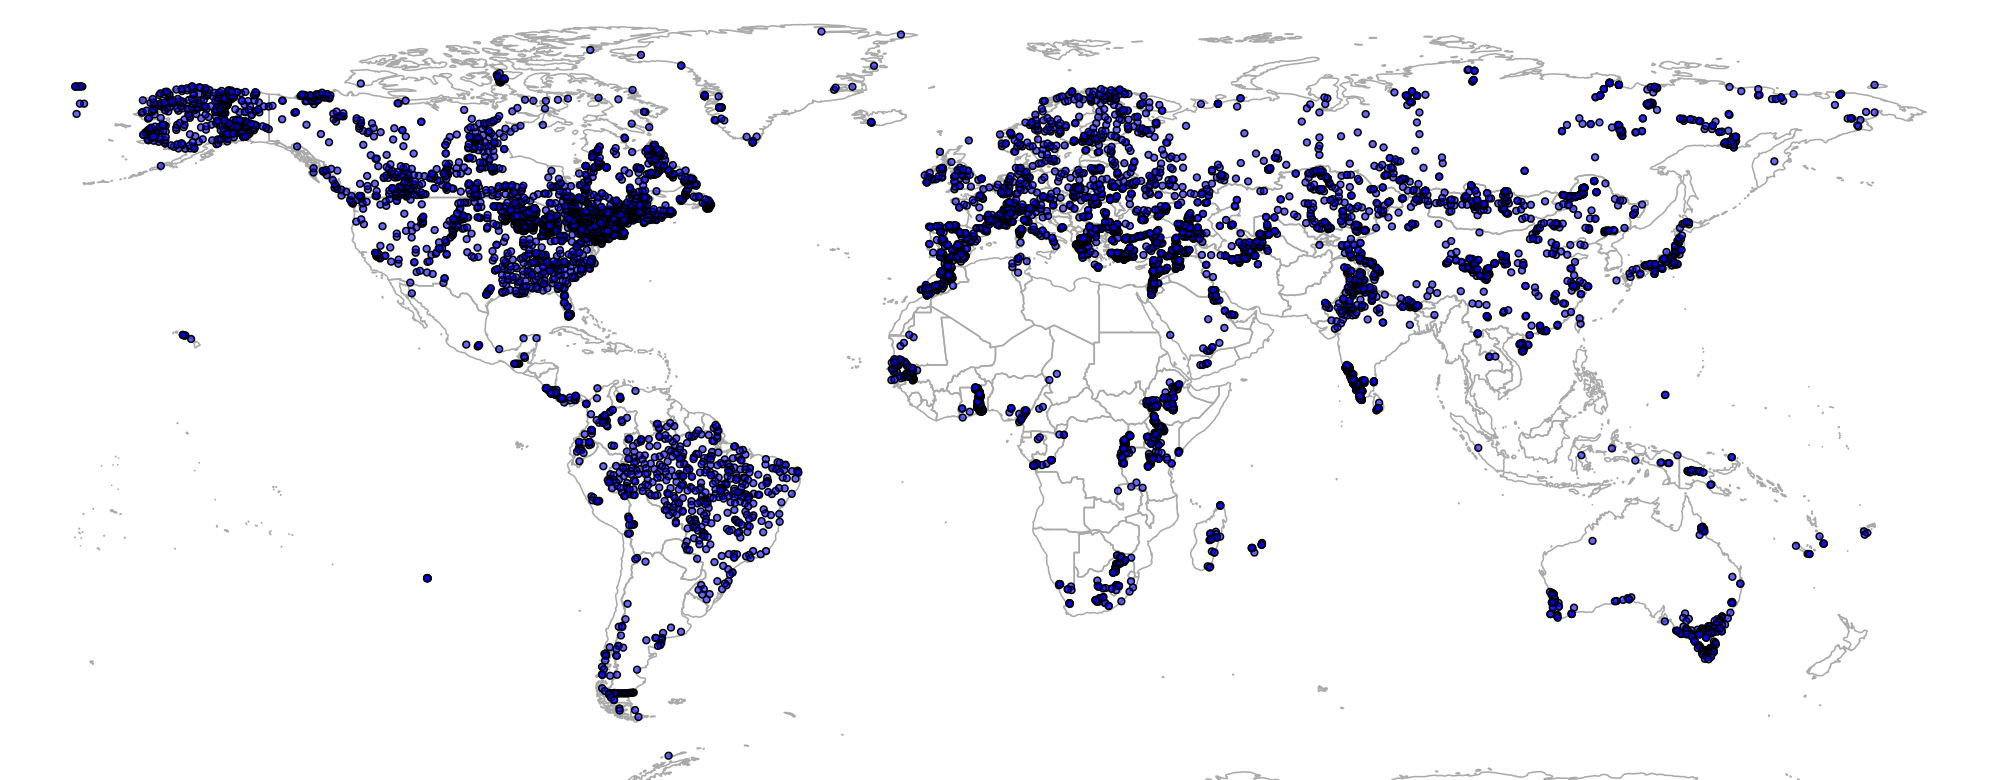
\includegraphics[width=\linewidth]{Fig_2.png}
\caption{Spatial distribution of BIOME 6000 training points. A total of 8057 unique locations are shown on the map.}
\label{Fig_biome_points_worldmap}
\end{figure}

Some sites in the BIOME 6000 data set have multiple reconstructions based on multiple nearby modern pollen samples (up to 30), which provides a useful measure of the reconstruction uncertainty, but could lead to modeling bias because the number of modern samples varies between sites. To reduce these unwanted effects, we use only the most frequently reconstructed biome at each site and for those sites with two equally common reconstructions (ca.\@ 900) we use both observations. \par

The number of biomes differentiated varies from region to region, and some biomes were only reconstructed in specific regions where they are particularly characteristic, although they may occur, but not be recognized, elsewhere. Furthermore, some biomes that can be recognized on the modern landscape were never reconstructed in the BIOME 6000 data set (e.g.\@ cushion forb tundra) --- either because of the sample distribution or because the characteristic plant-functional types were also spread amongst other biomes. Simplified or \emph{``megabiome''} classifications (e.g.\@ \citet{Harrison2012403}) involve a substantial loss of information. We have therefore created a new standardization of the classification scheme (see further Table~\ref{Table_Biome_results}; the final scheme has 20 globally applicable and distinctive biomes) which preserve the maximum number of distinct biomes that were reconstructed as present in multiple regions.\par

There are relatively few data vegetation reconstructions for tropical South America, which could lead to extrapolation problems and omission of important PNV classes in Latin America, but also potentially in tropical parts of Africa and Asia. To reduce under-representation of tropics, we have added 350 randomly simulated points based on the RADAM Brazil natural vegetation polygon map at high spatial detail (Radam Vegeta{\c{c}}{\~a}o SIRGAS map) \citep{veloso1992manual} obtained from \url{ftp://geoftp.ibge.gov.br/}. Before generating the pseudo-observations for Brazil, we translated SIRGAS map legends to match the BIOME 6000 classes. This translation is also available via the project's github repository. This gave a total of 8057 unique individual locations represented in the combined data set i.e.\@ a total of 8959 training observations (Fig.\@~\ref{Fig_biome_points_worldmap}).\par

We have mapped the distribution of biomes for all land pixels, with the exception of water bodies, barren land and permanent ice areas. Barren land and permanent ice areas were masked out using the ESA's global land cover maps for the period 2000--2015 (\url{https://www.esa-landcover-cci.org}) and the long-term FAPAR images, both available at relatively fine resolution of \SI{300}{\meter}. We only mask out pixels that are permanent ice/barren ground and have a FAPAR = 0 throughout the period 2000--2015.\par

\subsubsection*{European Forest Tree occurrence records}

For mapping PNV distribution of forest tree taxa (note: most of these are individual species, but some are only recognised at sub-genus or genus level) in Europe we have merged two point data sets: EU Forest \citep{mauri2017eu} (588,983 records covering 242 species) and GBIF occurrence records of the main forest tree taxa in Europe. The GBIF Occurrence data was downloaded on 23rd January 2017 (\url{http://dx.doi.org/10.15468/dl.fhucwx}). We focus on modeling just the 76 forest tree taxa indicated in the European Atlas of Forest Tree Species \citep{san2016european}. \par

\begin{figure}[ht]
\centering
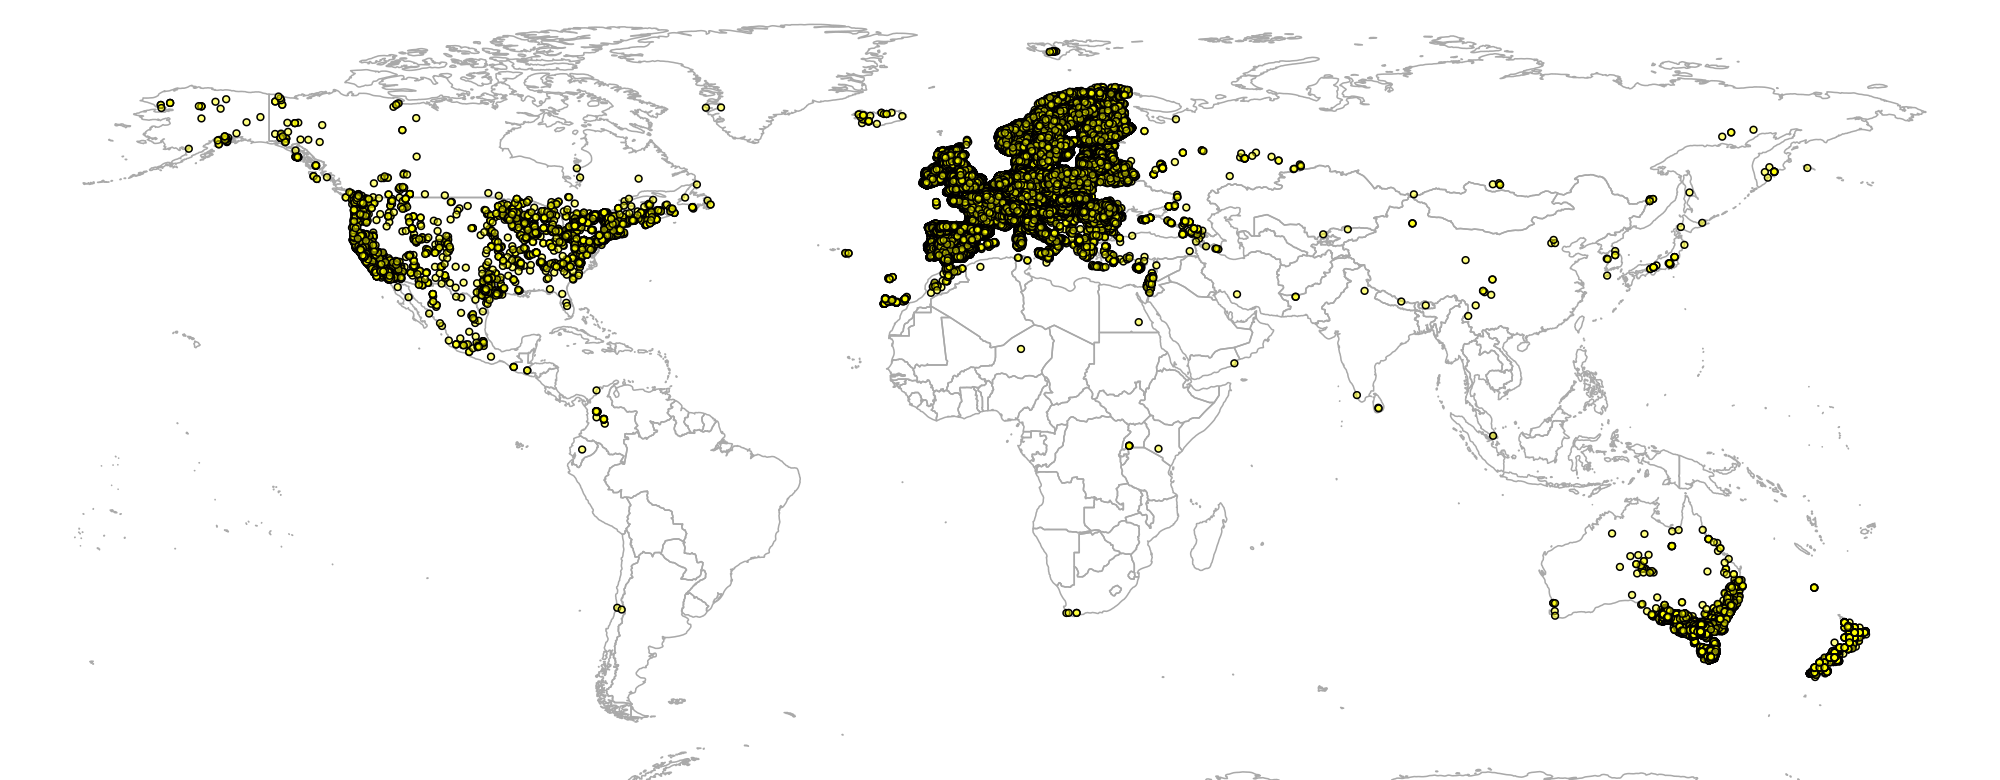
\includegraphics[width=\linewidth]{Fig_3.png}
\caption{Merge of EU Forest \citep{mauri2017eu} and GBIF occurrence records used to build models to predict PNV for the 76 forest tree taxa. Total of 1,546,435 shown on the map.}
\label{Fig_EU_forest_species_worldmap}
\end{figure}

Global GBIF occurrence data can be obtained by using the \textsf{rgbif} package, in which case the only important parameter is the \verb"taxonKey" (e.g.\@ \emph{``Betula spp.''} corresponds to GBIF taxon key \texttt{2875008}). After the bulk data download (which gives about 4 million occurrences), we imported all points and then subset occurrences based on the list of taxon keys and and coordinate uncertainty ($<$\SI{2}{\kilo\meter} positional error). This gave a total of 1,546,435 training points from which about 2/3 are GBIF points (Fig.\@~\ref{Fig_EU_forest_species_worldmap}). We assume in further analysis that the EU Forest point locations and representativeness are more trustworthy, hence we assign $4\times$ higher weights to these points than to the GBIF points. \par

Certain forest tree species (\emph{Chamaecyparis lawsoniana}, \emph{Eucalyptus globulus} and  \emph{Pseudotsuga menziesii}), that are shown in the European Atlas of Forest Tree Species are introduced i.e. planted and do not generally propagate naturally. Hence, they were removed from the list of target forest tree species. We retained, however, three species (\emph{Ailnthus altissima}, \emph{Picea sitchensis} and \emph{Robinia pseudoacacia}) that are not native but are extensively naturalized. The total number of target forest tree taxa was 73.\par

We built predictive models for European forest tree taxa using information on their global distribution, but only generate predictions for Europe. In other words, we use a global compilation for model training to increase the precision of the definition of the ecological niche of each taxon, but then predict only for Europe as the selection of taxa is based on the European Atlas of Forest Tree Species \citep{san2016european}. \par

\subsubsection*{FAPAR}

Fraction of Absorbed Photosynthetically Active Radiation (FAPAR) monthly images for 2014--2017 were obtained from \url{https://land.copernicus.eu} (original values reported in the range 0--235 with scaling factor 1/255 i.e.\@ with a maximum value of 0.94). From a total of 142 images downloaded from \url{https://land.copernicus.eu} we derived minimum, median and maximum value of FAPAR per month (12) using the \SI{95}{\percent} probability interval using the \textsf{data.table} package (\url{http://r-datatable.com}). For regression modeling we only report results of predictions of median values of FAPAR; predictions of minimum and maximum FAPAR can be obtained from the data repository.\par

\begin{figure}[!hbt]
\centering
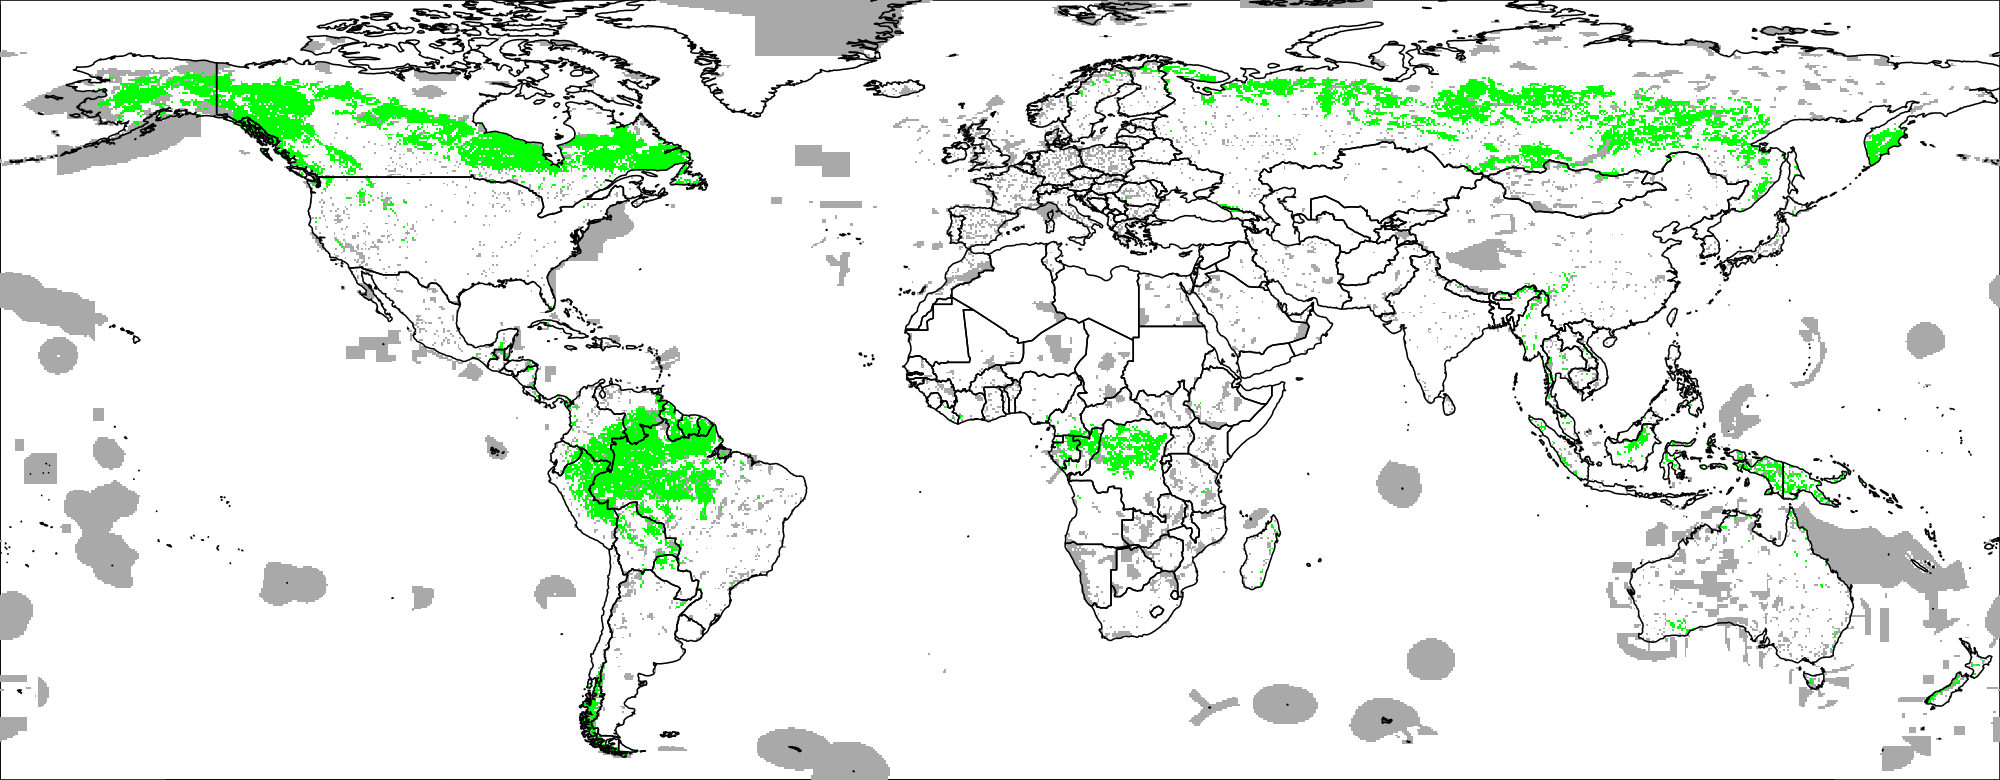
\includegraphics[width=\linewidth]{Fig_4.png}
\caption{World's Protected Areas (dark gray) based on \url{http://protectedplanet.net} and Intact Forest Landscapes for year 2000 (green) based on \url{http://intactforests.org}. These maps were used to randomly select some 30,000 training points to predict potential FAPAR under PNV.}
\label{Fig_intactareas_worldmap}
\end{figure}

We model median and upper \SI{95}{\percent} FAPAR values as a function of the same covariate layers used in all three case studies. For model training we use ca.\@ 30,000 randomly sampled points (Simple Random Sampling) exclusively from protected area as shown in the World Database on Protected Areas (WDPA) data set (\url{http://protectedplanet.net}) and the Intact Forest Landscapes (IFL) data set for 2000 and 2013 \citep{potapov2008mapping} Fig.\@~\ref{Fig_intactareas_worldmap}). We use about $3\times$ more training points from the IFL 2013 areas for model development than from the WDPA and IFL 2000 masks to emphasize more ecological conditions of intact vegetation.\par 

The prediction model for FAPAR under PNV is in the form of: 

\begin{Schunk}
\begin{Sinput}
R> FAPAR ~ cm + X1m + X2m + X3 + ... + Xp
\end{Sinput}
\end{Schunk}

\noindent where \verb"X1m" is the covariate with monthly values (for example precipitation, day-time and night-time temperatures etc), \verb"X3" is the environmental covariates that do not vary through year (e.g.\@ lithology or DEM derivatives), and \verb"cm" is the cosine of the month number:

\begin{equation}
c_m = \cos \left( \mu /12 \cdot 2 \cdot \pi \right)
\end{equation}

\noindent where $\mu$ is the month number 1--12. The total number of training observations used to build models is in fact 180,483 (each training site is represented up to 12 times).\par

For PNV FAPAR mapping we have masked out all water bodies including lakes and rivers, following the ESA's global land cover maps for the period 2000--2015 (\url{https://www.esa-landcover-cci.org}) and permanent ice/barren ground.\par

\subsection*{Input data: environmental covariates}

For modeling purposes, we use a stack of 160 spatially explicit co-variate data layers that represent standard ecological gradients essential for growth and survival of plants:

\begin{itemize}[noitemsep]
  \item DEM derivatives quantifying various landscape metrics and hydrological processes: slope, curvature, topographic index, topographic openness, valley depth and multi-resolution valley bottom index; all derived using the SAGA GIS \citep{gmd-8-1991-2015};
  \item Mean, minimum and maximum monthly temperatures derived as a mean between WorldClim v2 (\url{http://worldclim.org/version2}) and CHELSA climate \citep{karger2017climatologies}.
  \item Mean monthly precipitation images derived as a weighted average between the WorldClim v2, CHELSA climate and Global Precipitation Measurement Integrated Multi-satellitE Retrievals for GPM (IMERG) rainfall product.
  \item CHELSA Bioclimatic layers downloaded from \url{http://chelsa-climate.org/}, including: annual mean temperature, mean diurnal temperature range, isothermality (day-to-night temperature oscillations relative to the summer-to-winter oscillations), temperature seasonality (standard deviation of monthly temperature averages), maximum temperature of warmest month, minimum temperature of coldest month, temperature annual range, mean temperature of warmest quarter, mean temperature of coldest quarter, annual precipitation amount, precipitation of wettest month, precipitation of driest month, precipitation of wettest quarter, precipitation of driest quarter \citep{karger2017climatologies};
  \item European Space Agency's CCI-LC snow probability monthly averages based on MODIS snow products MOD10A2 downloaded from \url{http://maps.elie.ucl.ac.be/CCI/viewer/index.php};
  \item USGS Global Ecophysiography landform classification and lithological map at \SI{250}{\metre} resolution  obtained from \url{http://rmgsc.cr.usgs.gov/outgoing/ecosystems/Global/} and based on Global Lithological Map (GLiM) \citep{GGGE:GGGE2352};
  \item MODIS Cloud fraction monthly images obtained from \url{http://www.earthenv.org/cloud} \citep{WilsonJetz2016};
  \item Global Water Table Depth in meters based on \citet{fan2013global};
  \item NASA's monthly MODIS Precipitable Water Vapor images (\verb"MYDAL2_M_SKY_WV" data set at \url{http://neo.sci.gsfc.nasa.gov});
  \item Potential wetlands GIEMS map \citep{fluet2015development};
  \item Global Surface Water dynamics images: occurrence probability, surface water change, and water maximum extent; downloaded from \url{https://global-surface-water.appspot.com/download} \citep{pekel2016high};
  \item Density of earthquakes based on the USGS Earthquake Archives (\url{http://earthquake.usgs.gov/earthquakes/});
\end{itemize}

Some CHELSA bioclimatic layers contained too many missing pixels or artifacts (e.g.\@ mean temperature of wettest quarter, mean temperature of driest quarter, precipitation seasonality, precipitation of warmest quarter and precipitation of coldest quarter) and hence were not used for further modeling to avoid propagating those artifacts to final predictions. \par 

All original layers have been resampled to the standard grid at a spatial resolution of 1/120 decimal degrees (about \SI{1}{\kilo\metre}) covering latitudes between -62.0 and 87.37. Some layers such as Water Vapour needed to be downscaled from \SI{10}{\kilo\metre} to \SI{1}{\kilo\metre} resolution, for which we used the bicubic splines algorithm as implemented in GDAL \citep{mitchell2014geospatial}. We do not map Antarctica as this continent is dominantly covered with permanent ice and there are no training points. We limit all analysis to \SI{1}{\kilo\metre} i.e.\@ 1/120 degrees in geographical coordinates, to avoid too high of a computational load, even though many of environmental covariates are also available at finer resolutions. \par 

We use the same stack of covariates for mapping global distribution of biomes, FAPAR and forest tree species in Europe, in order to be able to compare model performance and investigate whether the most important covariates differ among the three case studies.\par

\subsection*{Machine Learning Algorithms (MLA) examined}

We examine predictive performance of the following MLA's:

\begin{itemize}
\item Neural networks \citep{Venables2002Springer},
\item Random forest \citep{breiman2001random,cutler2007random,Biau2016,peerj.preprints.26693v1},
\item Generalized Boosted Regression Models \citep{friedman2002stochastic},
\item K-nearest neighbors \citep{Venables2002Springer},
\end{itemize}

Neural networks are available from several packages in \textsf{R}. Here we use the \textsf{nnet} package \citep{Ripley2017nnet} also described in \citet{Venables2002Springer}. Random forest is efficiently implemented in the \textsf{ranger} package \citep{Wright2016} and can be used to to process large data sets. Generalized Boosted Regression Models are available via the \textsf{gbm} package \citep{ridgeway2010gbm}. The K-nearest Neighbour Regression is available via the \textsf{class} package i.e.\@ the \texttt{knn} function \citep{Venables2002Springer}. Of these four algorithms, the K-nearest neighbors is computationally the least intensive and results in relatively simple models, while random forest is computationally the most intensive and results in large models. However, a limitation of the K-nearest neighbors approach is that it does not handle high dimensional data in comparison to random forest or neural nets.\par

We also test using the same packages to fit models for regression-type problems (e.g.\@ modeling of FAPAR), with the exception of the \textsf{class} package i.e.\@ the \texttt{knn} function which can only be used for classification problems. For modeling FAPAR we instead added use of the Cubist approach, available via the \textsf{Cubist} package \citep{kuhn2014cubist}, and the Extreme Gradient Boosting approach available via the \textsf{xgboost} package \citep{Chen2016}.\par 

The \textsf{caret} package has many more MLA of interest for classification and regression problems than presented here, but many are not fully optimized for large data sets and hence also not applicable for large data sets ($\gg 1000$ observations with $\gg 100$ covariates).\par

\subsection*{Model selection}

For model fitting and model selection we use the \textsf{caret} package implementation for automated evaluation of models. When comparing performance of the models we look at classification accuracy based on cross-validation with refitting implemented in the \textsf{caret} package via the setting \citep{JSSv028i05,kuhn2013applied}:

\begin{Schunk}
\begin{Sinput}
R> ctrl <- trainControl(method="repeatedcv", number=5, repeats=2)
\end{Sinput}
\end{Schunk}

\noindent which translates as: models are refit 5 times using \SI{80}{\percent} of the data and predictions derived from the fitted models are compared with the remaining observations; this process is then repeated two times to produce stable results. The reported accuracy is the map accuracy (0--\SI{100}{\percent}) and/or Root Mean Square Error (RMSE) derived using all merged cross-validations \citep{JSSv028i05,kuhn2013applied}. Since most of the data sets are fairly large and model fitting can take hours, even in a High Performance Computing environment, we limit the number of repetitions to 2.\par

For FAPAR (regression modeling) and selection of the final prediction model we use the same repeated cross-validation as implemented via the \textsf{caret} package. This is, in principle, similar to evaluation of the classification accuracy, except the comparison criterion is RMSE.\par

All analyses were run on a High Performance Computing Amazon ec2 server with 64 threads (32 CPU's) and \SI{256}{\gibi\byte}~RAM. Total computing time to produce all outputs is about 12 hours of optimized computing (or about 600 CPU hours). \SI{1}{\kilo\metre} data can be processed with 2 degree tiles, which usually requires some 5000 tiles to represent the land mask. All processing steps and preparation of input and output maps are fully documented at \url{https://github.com/envirometrix/PNVmaps}. All output maps are available for download via \url{http://dx.doi.org/10.7910/DVN/QQHCIK} under the Open Database License (ODbL). \par

\subsubsection*{Performance of classification algorithms}

Performance of classification algorithms is assessed using 5--fold cross-validation with refitting of models. For evaluation of the mapping accuracy for biomes and tree species we use the map purity (0--\SI{100}{\percent}) and kappa metrics for the dominant (hard) classes as the key measures of predictive performance \citep{kuhn2013applied}. For each class we also provide predicted probabilities, which can be used to model transition zones and correlation between classes. For the predicted probabilities of class occurrences (0--1) we derived the True Positive Rate (TPR) and the Area Under the receiver operating characteristic Curve (AUC) as implemented in the \textsf{ROCR} package \citep{sing2005rocr,ROCR}. TPR value = 1 indicates a perfect match to the class positives in ground data while TPR values $<0.5$ can be considered poor mapping accuracy. Likewise, values of AUC close to 1 indicate high prediction performance, while values around 0.5 and below are considered poor. TPR and AUC provide probably a more informative measure of the mapping accuracy than overall mapping accuracy / kappa, as they also allow detection of problematic classes. \par

We also use Scaled Shannon Entropy Index, which can be derived using the per-class probability maps \citep{shannon1949communication,borda2011fundamentals}:

\begin{equation} \label{E:SSEI}
\mathsf{SSEI}_s(x) = -\sum_{i=1}^b{ P_i(x) \cdot \log_b P_i(x)} = \frac{ -\sum_{i=1}^b{ P_i(x) \cdot \log P_i(x)} }{ - b \cdot b^{-1} \cdot \log b^{-1} } 
\end{equation}

\noindent where $b$ is the total number of possible classes and $P$ is probability of class $i$. The Scaled Shannon Entropy Index ($\mathsf{SSEI}$) is in the range from 0--1, where 0 indicates a perfect classification and 1 (or \SI{100}{\percent}) indicates maximum confusion. Scaled Shannon Entropy Index should not be confused with classification accuracy assessment. For example, $\mathsf{SSEI}_s <$ \SI{60}{\percent} indicates relatively low confusion between classes i.e.\@ high accuracy, while mapping error of \SI{60}{\percent} would be considered a relatively poor classification accuracy result.\par

For the biomes data set, where spatial clustering of points is significant, we also use repeated spatial cross-validation as implemented in the \textsf{mlr} package \citep{mlr2016}: 

\begin{Schunk}
\begin{Sinput}
R> learner.rf = makeLearner("classif.ranger", predict.type = "prob")
R> resampling = makeResampleDesc("SpRepCV", fold = 5, reps = 5)
\end{Sinput}
\end{Schunk}

It has been shown that spatial autocorrelation in data and serious spatial clustering in training points can lead to somewhat biased estimate of the actual accuracy \citep{Brenning2012}. A solution to this problem is to apply spatial partitioning so that possible bias due to spatial proximity is minimized.\par

We also compare results of modeling potential distribution of tree species in Europe with the habitat type maps of Europe produced independently by \citet{san2016european} and \citet{brus2012statistical}. This comparison is visually based only.\par

\subsubsection*{Performance of regression algorithms}

Performance of regression algorithms is also assessed using 5--fold cross-validation with refitting of models. For assessment of the mapping accuracy for FAPAR we use as the main performance measures the root mean squared error (RMSE): 

\begin{equation} \label{E:RMSE}
{\rm RMSE} = \sqrt{\frac{ \sum_{j=1}^{m} [\hat y ({\bf s}_j) - y ({\bf s}_j)]^2 }{n}}
\end{equation}

\noindent and mean error (ME): 

\begin{equation} \label{E:ME}
{\rm ME} = \frac{\sum_{j=1}^{m} [\hat y ({\bf s}_j) - y ({\bf s}_j)]}{n} 
\end{equation}

\noindent where $\hat y ({\bf s}_j)$ is the predicted value of $y$ at the cross-validation location, and $m$ is total number of cross-validation points. We also report amount of variation explained by the model ($R^2$) derived as:

\begin{equation} \label{E:normvar}
 R^{2} = \left[ 1 - \frac{{\it{SSE}}}{{\it{SST}}} \right] \times 100\%
\end{equation}

\noindent where $\it{SSE}$ is the sum of squared errors at cross-validation points and $\it{SST}$ is the total sum of squares. A coefficient of determination close to 1 indicates a perfect model.\par

\section*{Results}

\subsection*{Global maps of biomes}

Results showed that a relatively accurate model of PNV could be produced from the BIOME 6000 data set using the existing stack of covariates at \SI{1}{\kilo\metre} spatial resolution. Results of cross-validation show the random forest (RF) model to be the best performing method and distinctively superior to all other approaches (Fig.\@~\ref{Fig_boxplot_biomes_accuracy}). The choice of the random forest \verb"mtry" parameter had little impact on overall accuracy, most likely because there was a high overlap in covariate maps so that even with smaller \verb"mtry" bagging the performance was relatively similar. The best prediction accuracy from among the four methods used for mapping global biomes was about \SI{68}{\percent}. The predicted biome classes are presented in Fig.\@~\ref{Fig_global_biomes_map}. \par 

\begin{figure}[!hbt]
\centering
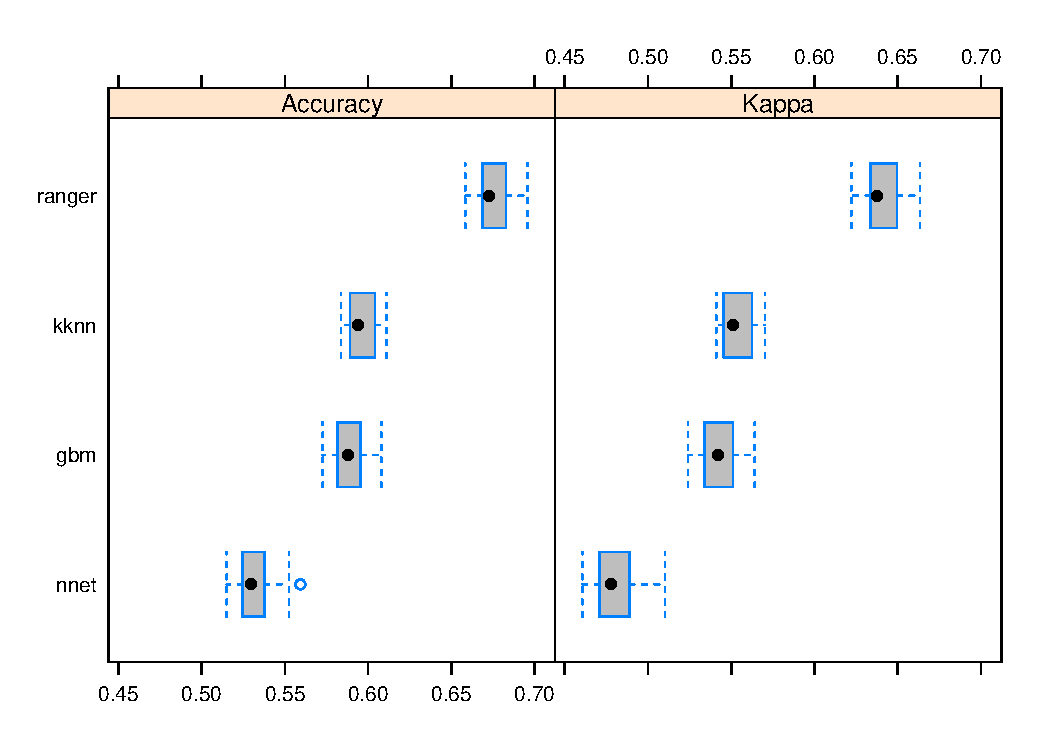
\includegraphics[width=.7\linewidth]{Fig_5.pdf}
\caption{Predictive performance of the target machine learning algorithms for mapping global distribution of biomes ($N=8653$; spatial distribution of training points is available in Fig.\@~\ref{Fig_biome_points_worldmap}). \textsf{ranger} = random forest, \textsf{kkn} = K-nearest neighbors, \textsf{gbm} = Generalized Boosted Regression Models, \textsf{nnet} = Neural networks.}
\label{Fig_boxplot_biomes_accuracy}
\end{figure}

\begin{figure}[!hp]
\centering
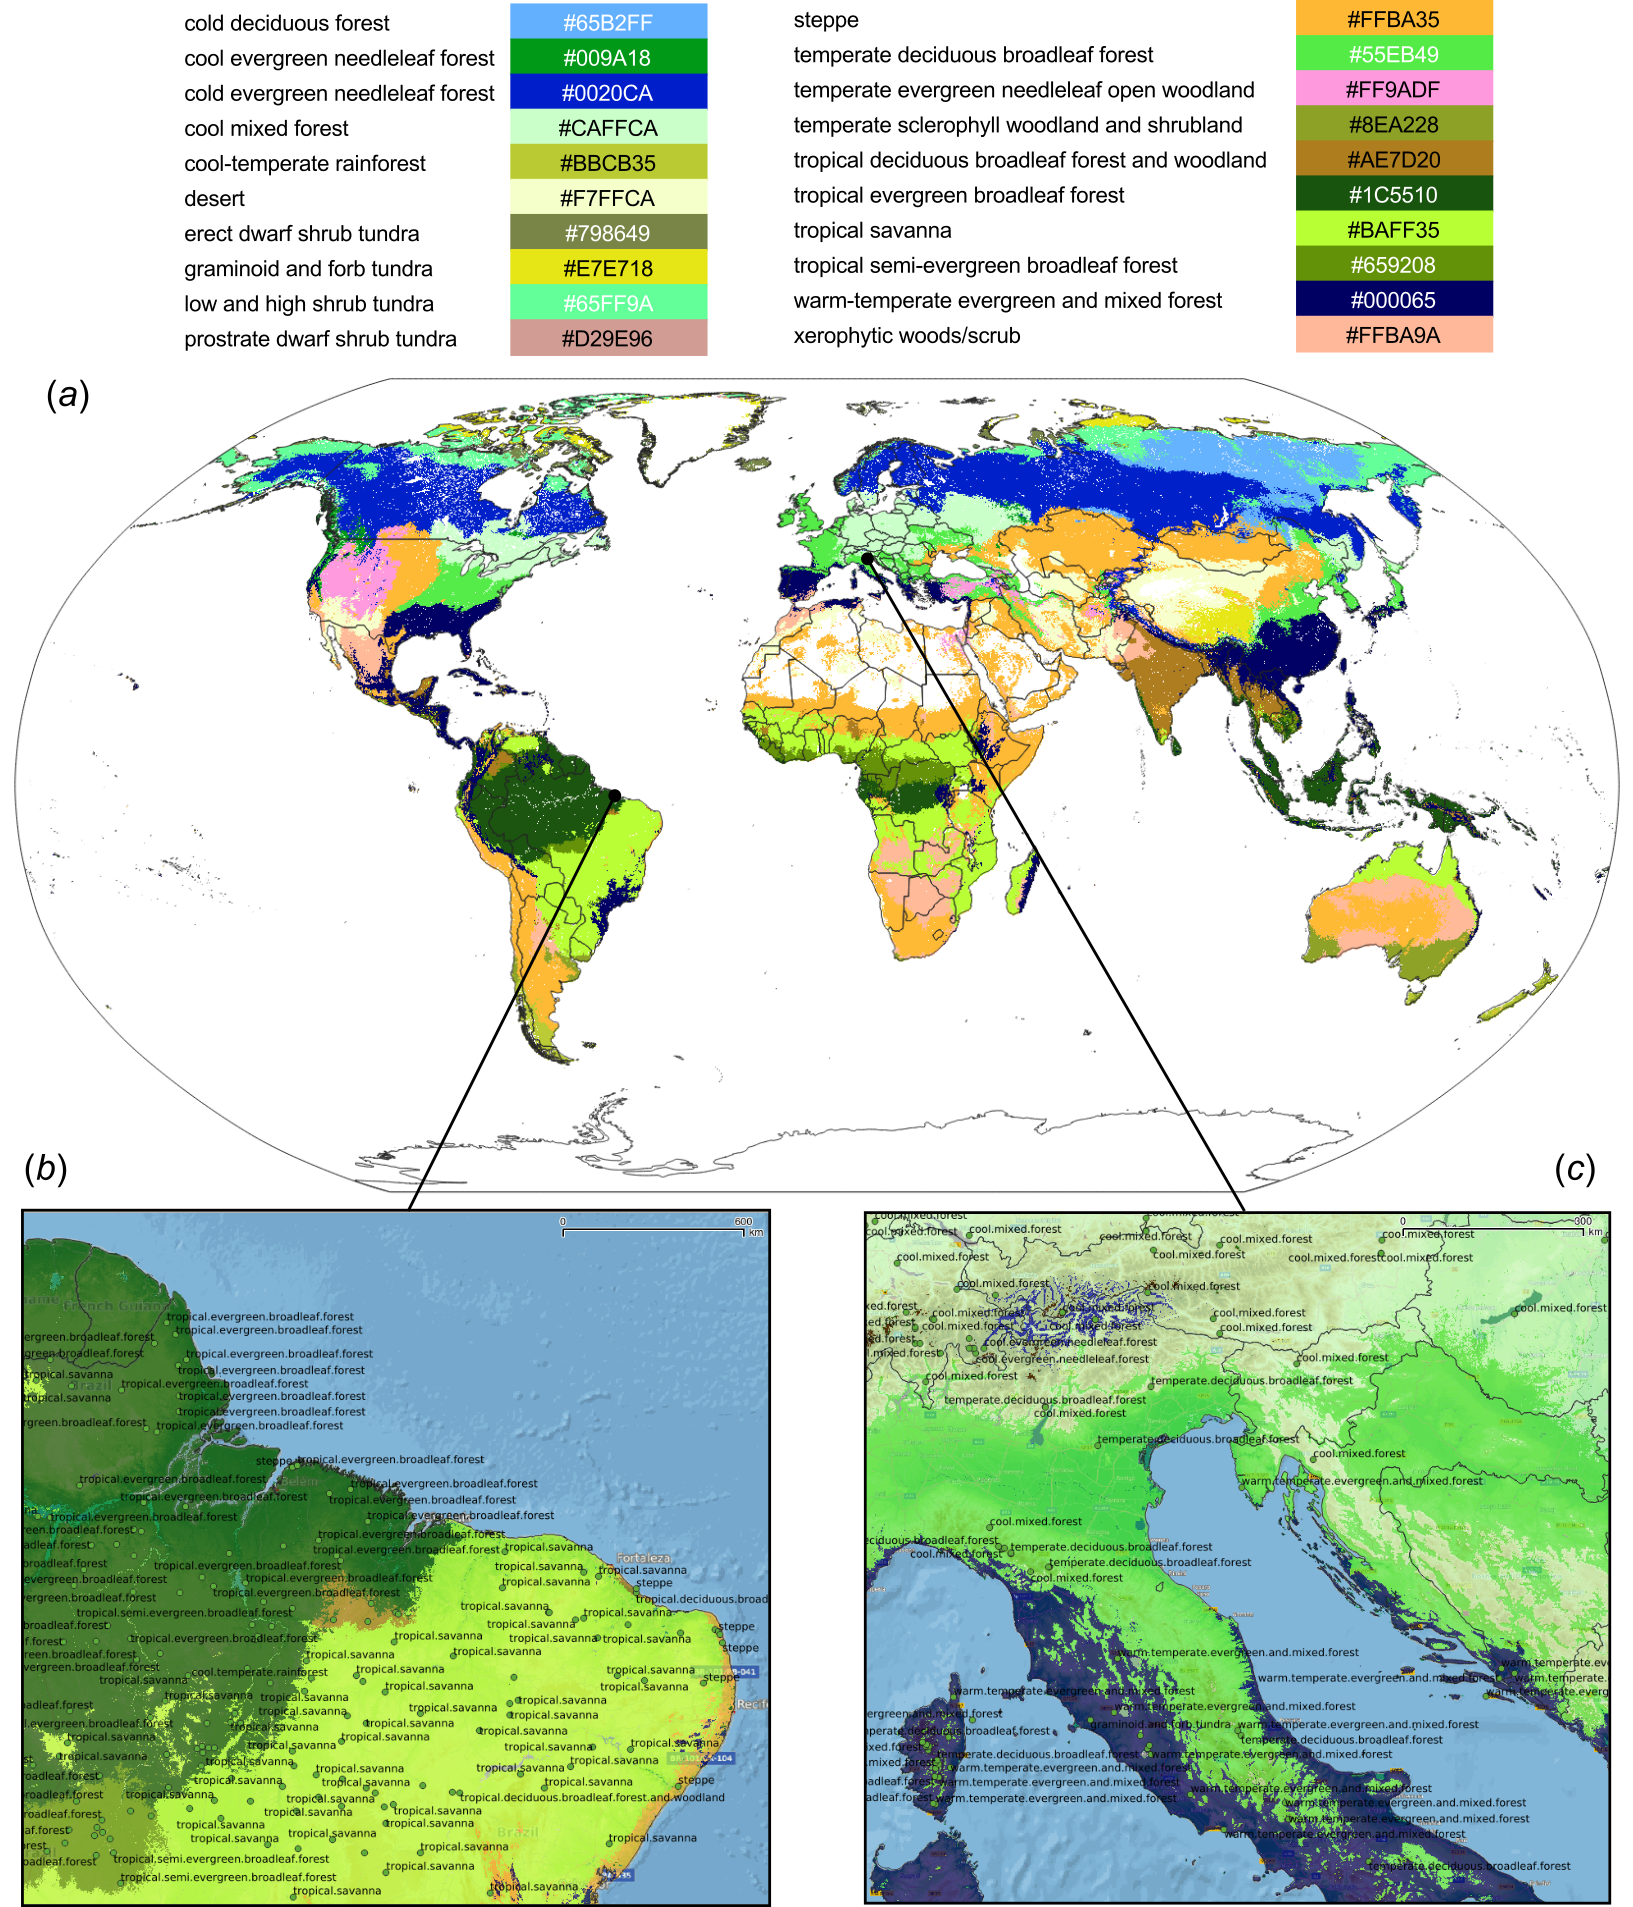
\includegraphics[width=\linewidth]{Fig_6.png}
\caption{Predicted PNV distribution for (a) global biomes with a zoom in on areas in Brazil (b) and Europe (c). Labels indicates training points from the BIOME 6000 data set (Fig.\@~\ref{Fig_biome_points_worldmap}). Background map data: Google, DigitalGlobe.}
\label{Fig_global_biomes_map}
\end{figure}

\begin{figure}[!hbt]
\centering
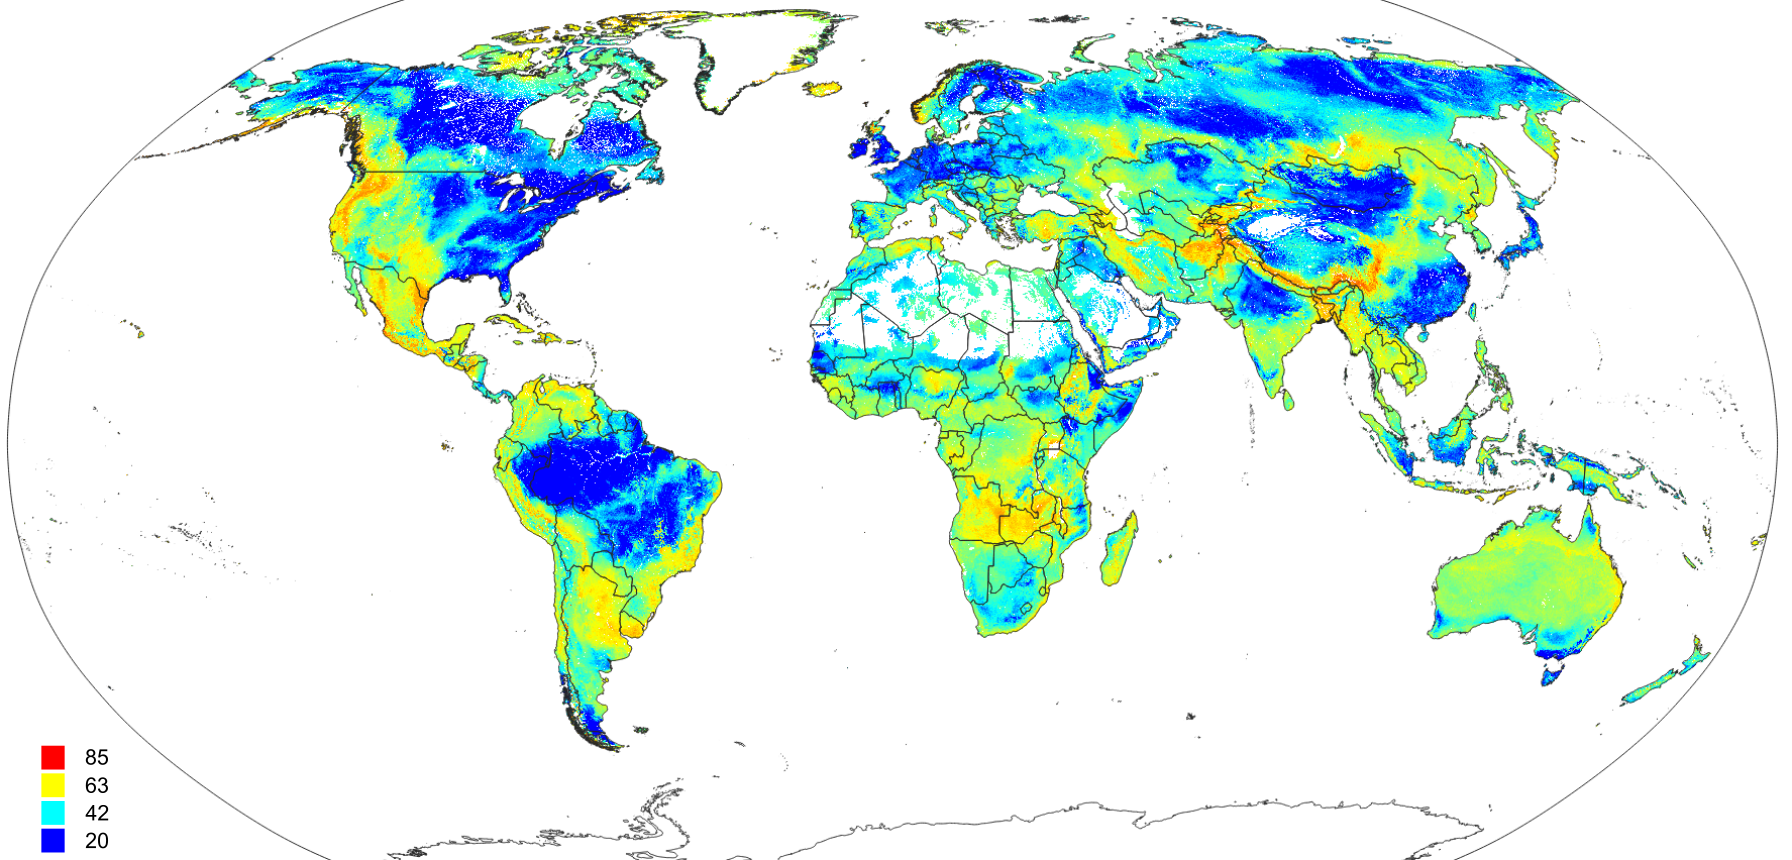
\includegraphics[width=\linewidth]{Fig_7.png}
\caption{Scaled Shannon Entropy Index (SSEI) derived using predicted probabilities for 20 biomes (classes) based on Eq.(\ref{E:SSEI}). High values of SSEI (red color) indicate high confusion between classes.}
\label{Fig_global_biomes_map_SSEI}
\end{figure}

\begin{table}[!hbt]
\centering
\caption{Summary results of cross-validation for mapping global distribution of biomes (20 classes). Classification accuracy for predicted class probabilities is based on 5--fold cross-validation with refitting. ME = \emph{``Mean Error''}, TPR = \emph{``True Positive Rate''}, AUC = \emph{``Area Under Curve''}, N = \emph{``Number of occurrences''}.}\label{Table_Biome_results}
\begin{tabular}{lrrrr}
\toprule
\textbf{Biome class}             & \textbf{ME} & \textbf{TPR}  & \textbf{AUC} & \textbf{N} \\
\midrule
cold deciduous forest                            & -0.01 & 0.89 & 0.96 & 201  \\
cold evergreen needleleaf forest                 & 0.01  & 0.87 & 0.98 & 892  \\
cool evergreen needleleaf forest                 & -0.07 & 0.87 & 0.93 & 201  \\
cool mixed forest                                & 0.01  & 0.86 & 0.97 & 1549 \\
cool temperate rainforest                        & 0.01  & 0.92 & 0.99 & 95   \\
desert                                           & 0.00  & 0.89 & 0.96 & 330  \\
erect dwarf shrub tundra                         & -0.01 & 0.89 & 0.98 & 145  \\
graminoid and forb tundra                        & -0.03 & 0.83 & 0.91 & 128  \\
low and high shrub tundra                        & -0.01 & 0.88 & 0.98 & 393  \\
prostrate dwarf shrub tundra                     & -0.02 & \textbf{0.54} & 0.90 & 11   \\
steppe                                           & 0.01  & 0.87 & 0.94 & 889  \\
temperate deciduous broadleaf forest             & -0.01 & 0.84 & 0.94 & 961  \\
temperate evergreen needleleaf open woodland     & 0.01  & 0.92 & 0.97 & 307  \\
temperate sclerophyll woodland and shrubland     & 0.00  & 0.94 & 0.99 & 154  \\
tropical deciduous broadleaf forest and woodland & 0.01  & 0.86 & 0.97 & 215  \\
tropical evergreen broadleaf forest              & 0.00  & 0.87 & 0.99 & 333  \\
tropical savanna                                 & 0.01  & 0.89 & 0.99 & 291  \\
tropical semi evergreen broadleaf.forest         & -0.05 & 0.87 & 0.98 & 160  \\
warm temperate evergreen and mixed forest        & 0.01  & 0.85 & 0.96 & 985  \\
xerophytic woods scrub                           & -0.02 & 0.88 & 0.95 & 388   \\     
\bottomrule
\end{tabular}
\end{table}

The most important covariates for the random forest model were: total annual precipitation, monthly temperatures, CHELSA bioclimatic layers, atmospheric water vapor images and monthly precipitation. Landform parameters and lithology are not amongst the top 20 most important predictors. The decline in variable importance was, however, gradual --- even lower ranked covariates might still affect the accuracy of predictions. \par

The detailed cross-validation results show that the only difficult class to predict was prostrate dwarf shrub tundra (Table~\ref{Table_Biome_results}). The TPR value for most class probabilities ranges from 0.83 to 0.94 indicating relatively high match with ground data. The Scaled Shannon Entropy Index map (Fig.\@~\ref{Fig_global_biomes_map_SSEI}) showed that the zones of highest confusion between classes can be found in Afghanistan, Nepal, mountainous parts of the USA and Mexico, parts of Angola and Zambia. The map of the SSEI is comparable to the confusion map produced by \citet{levavasseur2012statistical}, except in our case the Rocky Mountains in USA and mountains chains in South America show somewhat higher confusion. Many of the areas with high confusion index occur because the prediction model has problems distinguishing between closely-related biomes such as the \emph{``cold evergreen needleleaf forest''} and \emph{``cool evergreen needleleaf forest''} (e.g.\@ Scotland).\par

Results of the accuracy assessment based on the spatial Cross-Validation (\textsf{mlr} package implementation \citep{mlr2016}) further indicate that the spatial clustering of points does have a large effect on the mapping accuracy: spatial CV drops from 0.68 to 0.33 and weighted kappa to 0.45. This likely happens due to high spatial clustering of the biome points and due to the high spatial autocorrelation of biomes.  \par

\subsection*{European forest tree species}

The results of 5--fold cross validation with re-fitting at each fold, confirms that random forest was also the best prediction method for the forest taxa data set (Fig.\@~\ref{Fig_boxplot_EU_forest_accuracy}). The overall mapping accuracy was significantly lower than for biomes, but this reduction in accuracy was to be expected as many of these taxa occur in communities, resulting in natural overlap of forest tree taxa distribution. The mapping accuracy of individual taxa, however, can be relatively high with TPR values of between 0.16--0.90 and an average value of around 0.69 (Table~\ref{Table_EU_tree_species}). The final maps (Fig.\@~\ref{Fig_EU_forest_species_map}) showed a relatively good match with ground data, meaning that with the exception of some species of rarer occurrence (\emph{Picea omorika}, \emph{Cupressus sempervirens}, \emph{Prunus mahaleb}), the species probability distribution maps were relatively accurate. \par

\begin{figure}[!hbt]
\centering
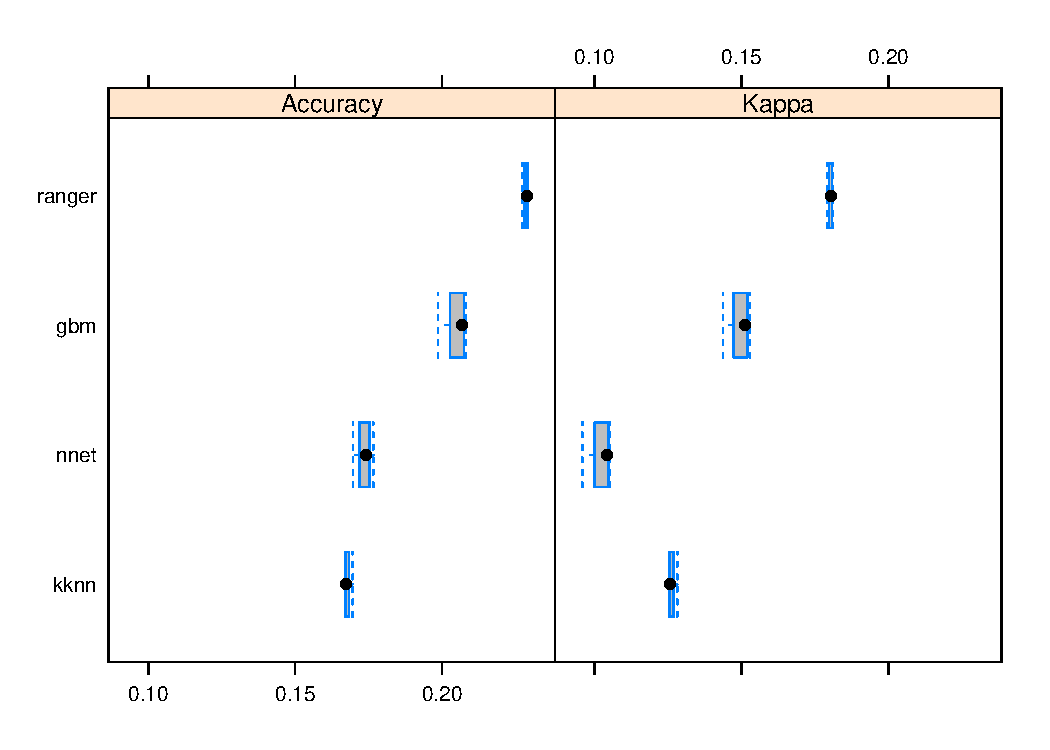
\includegraphics[width=.7\linewidth]{Fig_8.pdf}
\caption{Predictive performance of the target machine learning algorithms for mapping forest tree species ($N=$1.5 million distribution of training points is available in Fig.\@~\ref{Fig_EU_forest_species_worldmap}). \textsf{ranger} = random forest, \textsf{gbm} = Generalized Boosted Regression Models, \textsf{nnet} = Neural networks, \textsf{kkn} = K-nearest neighbors.}
\label{Fig_boxplot_EU_forest_accuracy}
\end{figure}

\begin{figure}[!hbt]
\centering
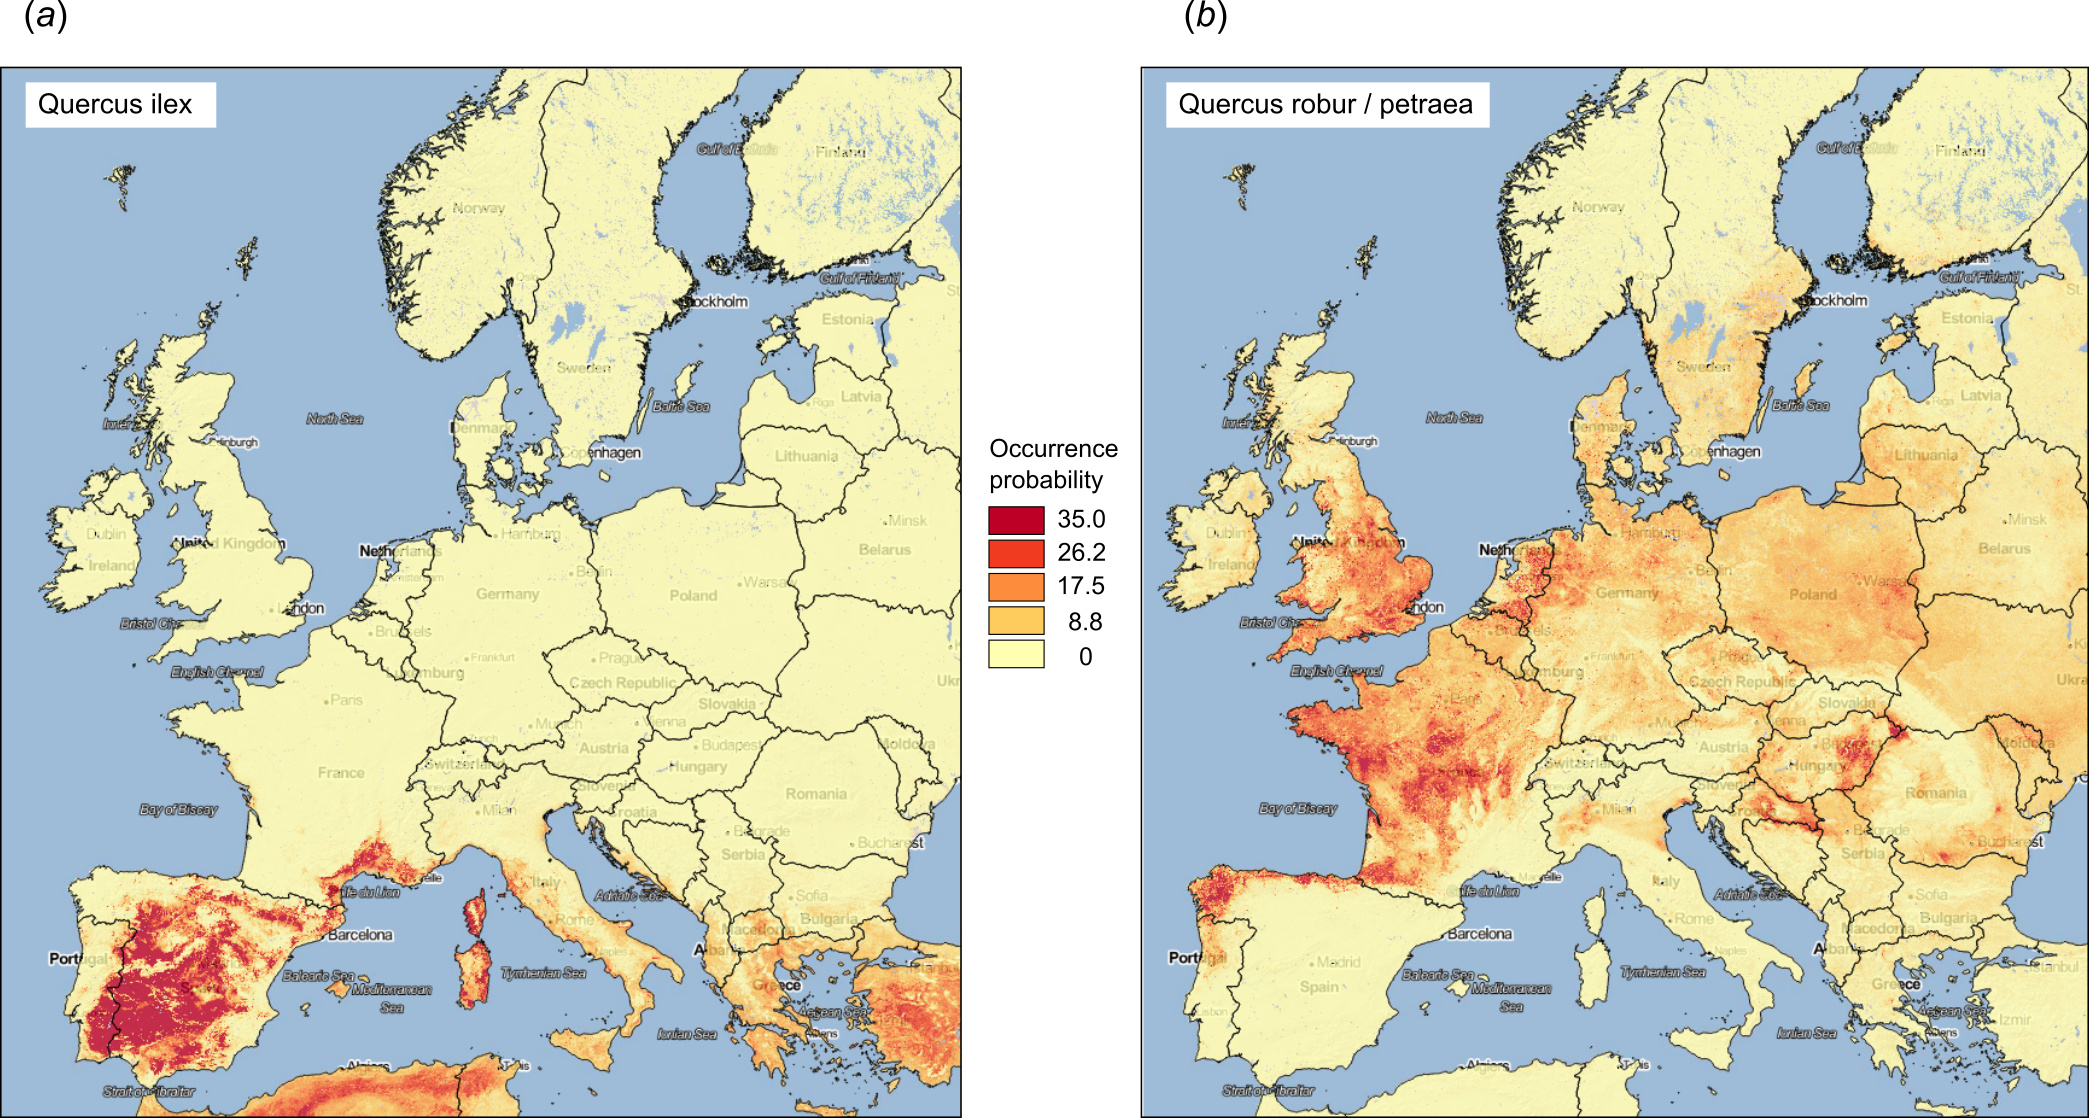
\includegraphics[width=\linewidth]{Fig_9.png}
\caption{Examples of predicted PNV distributions (probabilities) for European forest tree species (a) \emph{Quercus Ilex} (GBIF ID: 2879098; 36,724 training points) and (b) \emph{Quercus robur / petraea} (GBIF ID: 2878688; 404,296 training points). Background map data: Google, DigitalGlobe.}
\label{Fig_EU_forest_species_map}
\end{figure}

\begin{figure}[!hbt]
\centering
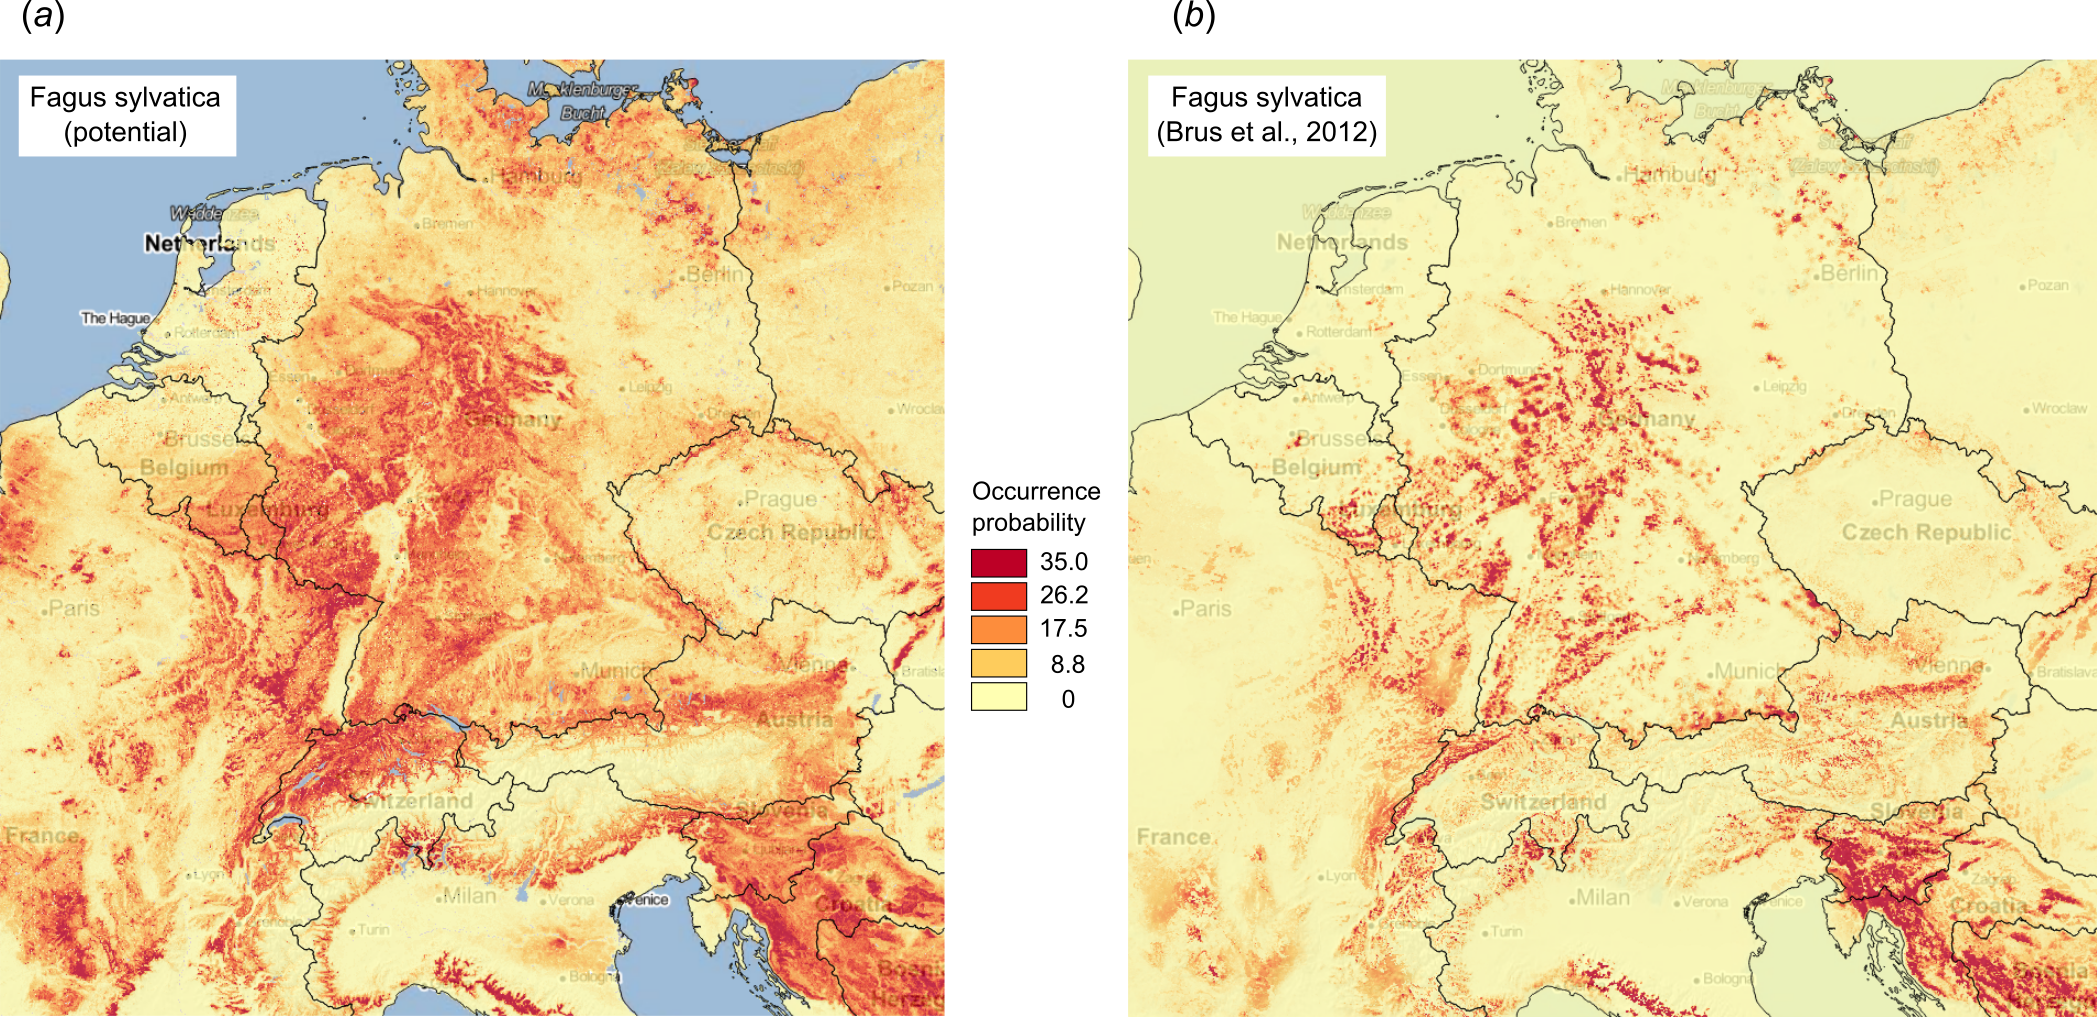
\includegraphics[width=\linewidth]{Fig_10.png}
\caption{Comparison between predicted PNV distribution for (a) \emph{Fagus sylvatica} (GBIF ID: 2882316) based on our results, and (b) based on the maps generated by \citet{brus2012statistical} i.e.\@ showing the presumed actual distribution of the tree species. Background map data: Google, DigitalGlobe.}
\label{Fig_EU_forest_Fagus_sylvatica}
\end{figure}

\begingroup
\renewcommand\arraystretch{0.6}
\begin{center}
\begin{longtable}{lrrrrr}
\caption{Results of cross-validation for the forest tree taxa. Classification accuracy for predicted class probabilities based on 5--fold cross-validation. ME = \emph{``Mean Error''}, TPR = \emph{``True Positive Rate''}, AUC = \emph{``Area Under Curve''}, N = \emph{``Number of occurrences''}. Taxa with less than $<50$ observations were omitted from analysis.}\label{Table_EU_tree_species} %% \vspace*{8mm} 
\\
\toprule
\textbf{Species name} & \textbf{GBIF taxon ID} & \textbf{ME} & \textbf{TPR}  & \textbf{AUC} & \textbf{N} \\  
\endfirsthead
\multicolumn{5}{c}
{\tablename\ \thetable\ -- \textit{Continued from previous page}} \\
\toprule
\textbf{Species name} & \textbf{GBIF taxon ID} & \textbf{ME} & \textbf{TPR} & \textbf{AUC} & \textbf{N} \\ 
\midrule
\endhead
\hline \multicolumn{5}{r}{\textit{Continued on next page}} \\
\endfoot
\hline
\endlastfoot
\midrule
\emph{Abies alba}                        & 2685484 & -0.01 & 0.77 & 0.92 & 16,150  \\
\emph{Acer campestre}                    & 3189863 & -0.01 & 0.65 & 0.83 & 19,819  \\
\emph{Acer platanoides}                  & 3189846 & -0.02 & 0.68 & 0.82 & 30,801  \\
\emph{Acer pseudoplatanus}               & 3189870 & -0.01 & 0.69 & 0.79 & 65,039  \\
\emph{Aesculus hippocastanum}            & 3189815 & -0.01 & 0.59 & 0.85 & 8,088   \\
\emph{Ailanthus altissima}               & 3190653 & 0.04  & 0.69 & 0.92 & 1,576   \\
\emph{Alnus cordata}                     & 2876607 & 0.05  & 0.73 & 0.95 & 904     \\
\emph{Alnus glutinosa}                   & 2876213 & 0.00  & 0.71 & 0.77 & 91,292  \\
\emph{Alnus incana}                      & 2876388 & -0.03 & 0.76 & 0.95 & 6,873   \\
\emph{Betula spp.}                       & 2875008 & -0.03 & 0.63 & 0.83 & 7,313   \\
\emph{Carpinus betulus}                  & 2875818 & 0.00  & 0.75 & 0.89 & 22,765  \\
\emph{Carpinus orientalis}               & 2875780 & 0.07  & \textbf{0.21} & 0.92 & 284     \\
\emph{Castanea sativa}                   & 5333294 & 0.00  & 0.74 & 0.91 & 13,049  \\
\emph{Celtis australis}                  & 2984492 & -0.01 & 0.54 & 0.92 & 594     \\
\emph{Cornus mas}                        & 3082263 & 0.03  & 0.51 & 0.90 & 827     \\
\emph{Cornus sanguinea}                  & 3082234 & -0.03 & 0.59 & 0.82 & 8,837   \\
\emph{Corylus avellana}                  & 2875979 & -0.02 & 0.67 & 0.76 & 48,140  \\
\emph{Cupressus sempervirens}            & 2684030 & -0.04 & \textbf{0.21} & 0.70 & 284     \\
\emph{Euonymus europaeus}                & 3169131 & -0.02 & 0.61 & 0.83 & 12,119  \\
\emph{Fagus sylvatica}                   & 2882316 & 0.00  & 0.73 & 0.81 & 89,044  \\
\emph{Frangula alnus}                    & 3039454 & -0.02 & 0.71 & 0.86 & 26,873  \\
\emph{Fraxinus angustifolia}             & 7325877 & -0.05 & 0.63 & 0.94 & 1,757   \\
\emph{Fraxinus excelsior}                & 3172358 & 0.00  & 0.67 & 0.74 & 91,111  \\
\emph{Fraxinus ornus}                    & 3172347 & 0.02  & 0.86 & 0.99 & 2,765   \\
\emph{Ilex aquifolium}                   & 5414222 & -0.01 & 0.66 & 0.82 & 26,873  \\
\emph{Juglans regia}                     & 3054368 & -0.03 & 0.60 & 0.89 & 3,643   \\
\emph{Juniperus communis}                & 2684709 & -0.03 & 0.71 & 0.86 & 21,189  \\
\emph{Juniperus oxycedrus}               & 2684451 & -0.07 & 0.71 & 0.97 & 1,705   \\
\emph{Juniperus phoenicea}               & 2684640 & -0.07 & 0.74 & 0.98 & 1,137   \\
\emph{Juniperus thurifera}               & 2684528 & -0.03 & 0.87 & 0.99 & 1,886   \\
\emph{Larix decidua}                     & 2686212 & -0.01 & 0.71 & 0.89 & 15,581  \\
\emph{Olea europaea}                     & 5415040 & 0.00  & 0.90 & 0.99 & 7,080   \\
\emph{Ostrya carpinifolia}               & 5332305 & 0.06  & 0.90 & 0.99 & 1,809   \\
\emph{Picea abies}                       & 5284884 & 0.02  & 0.76 & 0.86 & 122,713 \\
\emph{Picea sitchensis}                  & 5284827 & 0.05  & 0.80 & 0.96 & 13,023  \\
\emph{Pinus cembra}                      & 5285134 & -0.01 & 0.77 & 0.96 & 853     \\
\emph{Pinus halepensis and Pinus brutia} & 5285604 & 0.03  & 0.86 & 0.99 & 16,951  \\
\emph{Pinus mugo}                        & 5285385 & 0.00  & 0.85 & 0.98 & 6,667   \\
\emph{Pinus nigra}                       & 5284809 & 0.01  & 0.79 & 0.93 & 13,540  \\
\emph{Pinus pinaster}                    & 5285565 & 0.01  & 0.86 & 0.98 & 17,080  \\
\emph{Pinus pinea}                       & 5285165 & -0.04 & 0.85 & 0.99 & 4,910   \\
\emph{Pinus sylvestris}                  & 5285637 & 0.02  & 0.78 & 0.85 & 153,928 \\
\emph{Populus alba}                      & 3040233 & -0.01 & 0.54 & 0.86 & 4,522   \\
\emph{Populus nigra}                     & 3040227 & -0.01 & 0.65 & 0.89 & 5,478   \\
\emph{Populus tremula}                   & 3040249 & -0.02 & 0.66 & 0.74 & 44,057  \\
\emph{Prunus avium}                      & 3020791 & -0.01 & 0.63 & 0.77 & 25,711  \\
\emph{Prunus cerasifera}                 & 3021730 & 0.00  & 0.73 & 0.94 & 3,928   \\
\emph{Prunus mahaleb}                    & 3022789 & -0.01 & \textbf{0.31} & 0.75 & 517     \\
\emph{Prunus padus}                      & 3021037 & -0.03 & 0.63 & 0.78 & 21,705  \\
\emph{Prunus spinosa}                    & 3023221 & -0.01 & 0.69 & 0.81 & 31,783  \\
\emph{Quercus cerris}                    & 2880580 & 0.00  & 0.80 & 0.97 & 4,109   \\
\emph{Quercus ilex}                      & 2879098 & 0.02  & 0.85 & 0.99 & 22,972  \\
\emph{Quercus pubescens}                 & 2881283 & 0.01  & 0.86 & 0.98 & 9,096   \\
\emph{Quercus pyrenaica}                 & 2878826 & 0.00  & 0.88 & 0.99 & 6,253   \\
\emph{Quercus robur and Quercus petraea} & 2878688 & 0.01  & 0.69 & 0.76 & 141,938 \\
\emph{Quercus suber}                    & 2879411 & -0.04 & 0.86 & 0.99 & 5,504   \\
\emph{Robinia pseudoacacia}              & 5352251 & 0.01  & 0.71 & 0.90 & 13,411  \\
\emph{Salix alba}                        & 5372513 & 0.02  & 0.72 & 0.90 & 11,938  \\
\emph{Salix caprea}                      & 5372952 & -0.03 & 0.68 & 0.78 & 40,879  \\
\emph{Sambucus nigra}                    & 2888728 & 0.00  & 0.70 & 0.81 & 44,961  \\
\emph{Sorbus aria}                       & 3012680 & -0.01 & 0.59 & 0.87 & 5,426   \\
\emph{Sorbus aucuparia}                  & 3012167 & -0.01 & 0.70 & 0.76 & 86,977  \\
\emph{Sorbus domestica}                  & 3013206 & -0.04 & \textbf{0.48} & 0.87 & 801     \\
\emph{Sorbus torminalis}                 & 3012567 & -0.03 & 0.62 & 0.92 & 2,558   \\
\emph{Taxus baccata}                     & 5284517 & -0.02 & 0.58 & 0.82 & 8,062   \\
\emph{Tilia spp.}                        & 3152041 & -0.02 & 0.50 & 0.82 & 4,393   \\
\emph{Ulmus spp.}                       & 2984510 & -0.03 & 0.64 & 0.92 & 5,426   \\
\emph{Tilia spp.}                        & 3152041 & 0.00  & 0.58 & 0.85 & 4,522   \\
\emph{Ulmus spp.}                        & 2984510 & -0.02 & 0.69 & 0.91 & 5,375  \\   
\bottomrule
\end{longtable}
\end{center}
\endgroup

The most important predictors in the random forest model for forest tree taxa were mean annual daily temperature, other monthly temperatures, elevation, CHELSA bioclimatic images, monthly precipitation and MODIS cloud fraction images. Covariates for lithology and landform classification did not feature in the top 20 predictors. It could be that the Global Lithological Map (GLiM) \citep{GGGE:GGGE2352}, which was used to represent changes in lithology, is too general for this scale of work. \par

Fig.\@~\ref{Fig_EU_forest_Fagus_sylvatica} illustrates differences between the map of actual distribution of \emph{Fagus sylvatica}, generated by \citet{brus2012statistical}, and our predictions. In this case, the potential for extending habitat of \emph{Fagus sylvatica} is significant, especially over parts of France and Germany.\par

Correlation analysis using all predicted distribution maps (matrix of Pearson's rho rank correlation coefficients for all possible pairs) indicated that many forest species are positively correlated, especially \emph{Fagus sylvatica} and \emph{Abies alba} and \emph{Populus nigra} and \emph{Salix alba}. High overlap between species probability maps reflects co-existence within communities, and thus could help with objectively defining forest communities.\par 

\newpage
\subsection*{Global monthly FAPAR}

The random forest approach also produced the best preditcions of potential FAPAR  (Fig.\@~\ref{Fig_boxplot_FAPAR_accuracy}). The models for FAPAR were highly significant with R-squared around \SI{90}{\percent} and RMSE at $\pm 24$ (original values in the range 0--232 where 235 corresponds to FAPAR=\SI{100}{\percent}) for the most accurate model based on 5--fold Leave-Location-Out cross-validation. However, unlike with biomes and forest species distributions, the regression-tree Cubist model achieves equal performance to that of random forest. The most important covariates for predicting FAPAR were total annual precipitation, MODIS cloud fraction images, CHELSA bioclimatic images, and monthly precipitation images. The \textsf{caret} package further suggested that \verb"mtry" parameter for Random Forest needs to be set higher than the default values for modeling FAPAR. Setting up \verb"mtry" $>$25 helps reduce the RMSE by about 7--\SI{8}{\percent}. \par

\begin{figure}[!hbt]
\centering
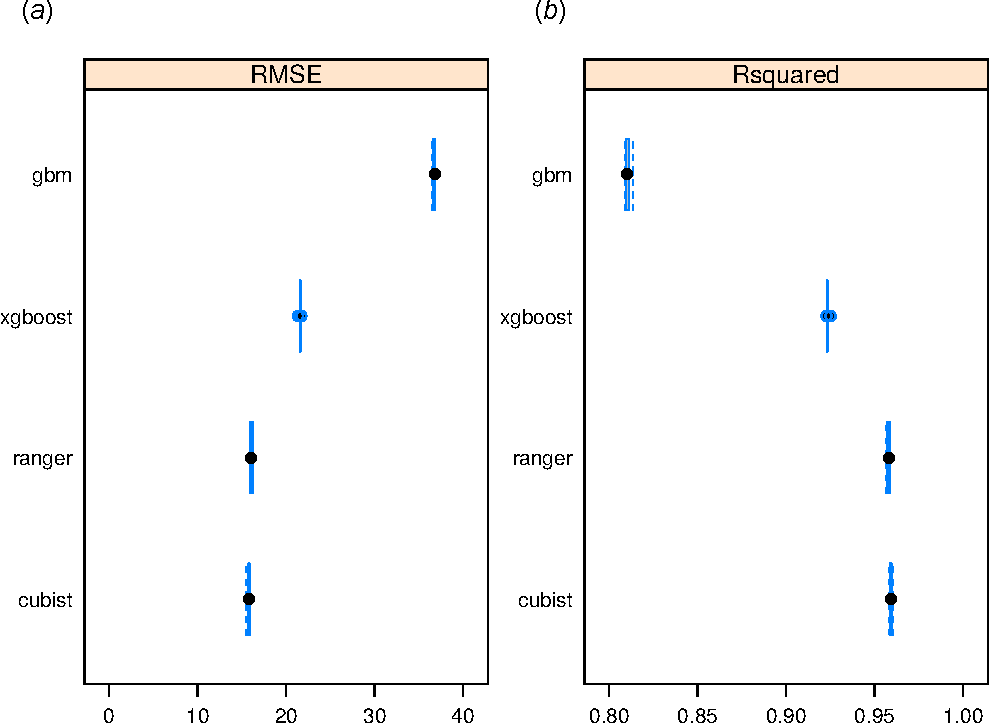
\includegraphics[width=.7\linewidth]{Fig_11.pdf}
\caption{Predictive performance of four machine learning algorithms for mapping global distribution of FAPAR ($N=180,990$). \textsf{gbm} = Generalized Boosted Regression Models, \textsf{xgboost} = Extreme Gradient Boosting, \textsf{ranger} = random forest,  \textsf{cubist} = Cubist Regression Models. (a) RMSE = Root Mean Square Error, (b) R-squared.}
\label{Fig_boxplot_FAPAR_accuracy}
\end{figure}

\begin{figure}[!hp]
\centering
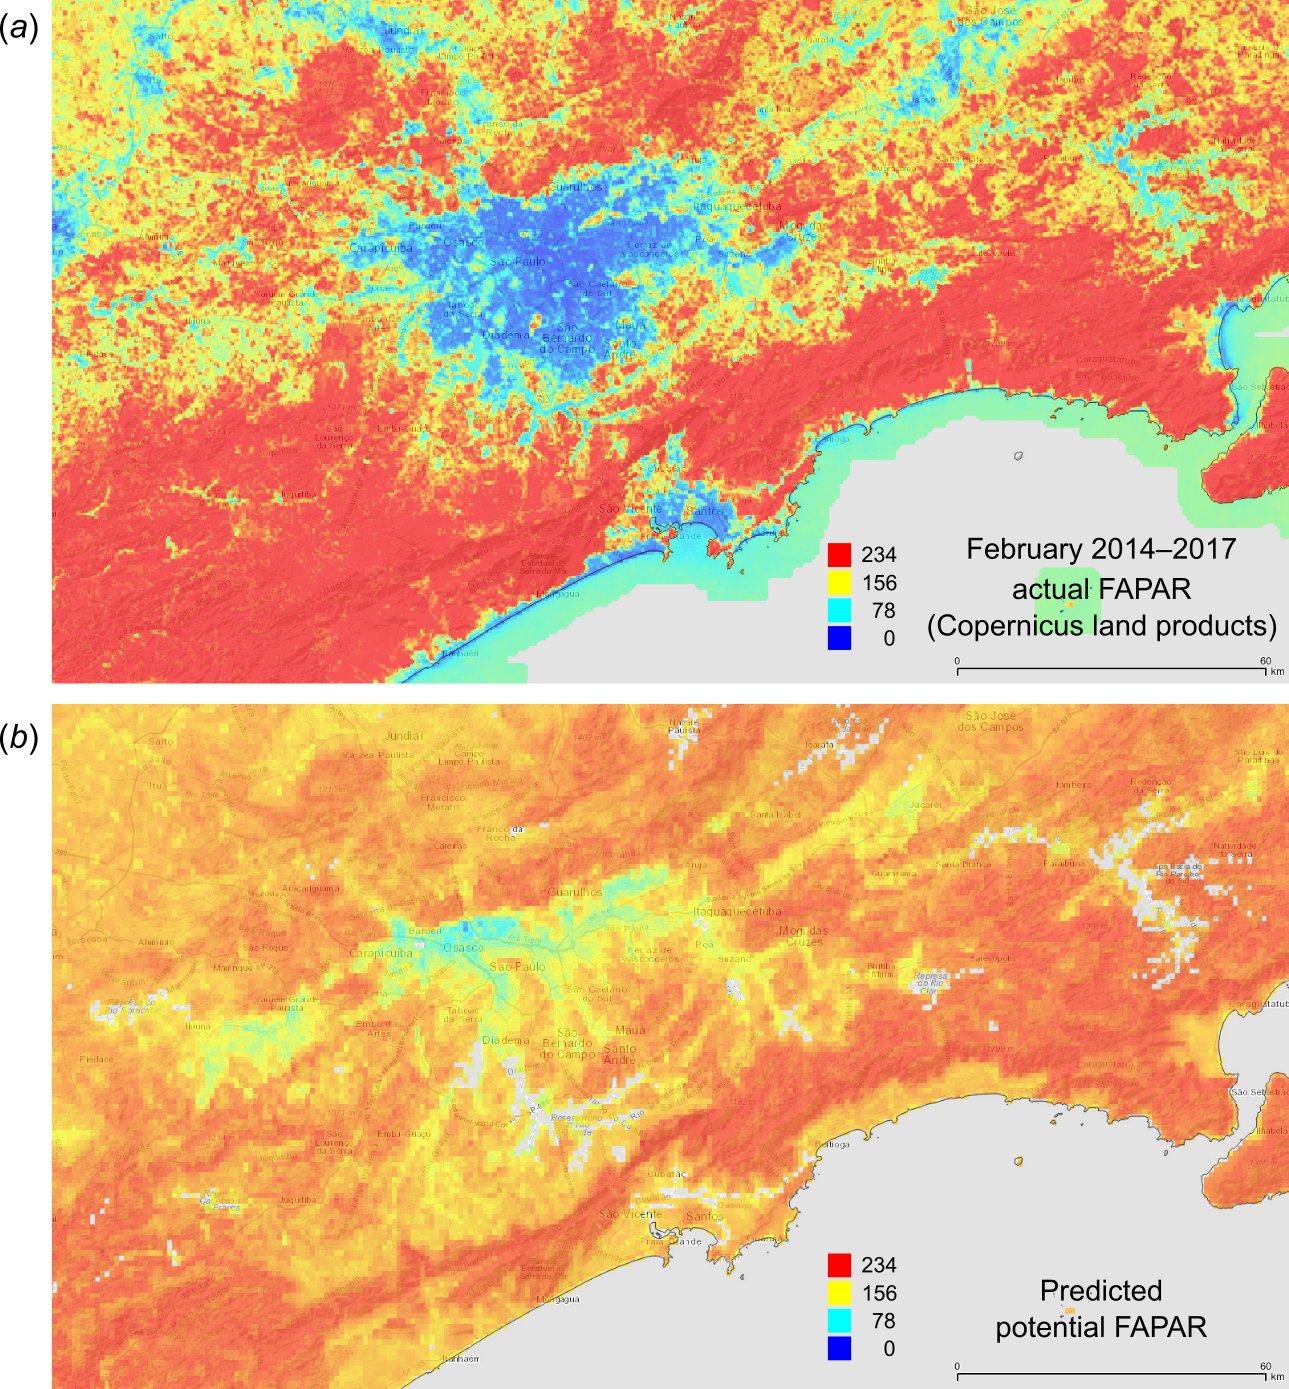
\includegraphics[width=\linewidth]{Fig_12.png}
\caption{FAPAR values for February based on the PNV samples: (a) actual (\SI{250}{\metre} resolution) and (b) predicted (\SI{1}{\kilo\metre} resolution). A zoom in area around the city of S\~{a}o Paulo in Brazil.}
\label{Fig_FAPAR_predicted_Sao_Paolo}
\end{figure}

\begin{figure}[!hp]
\centering
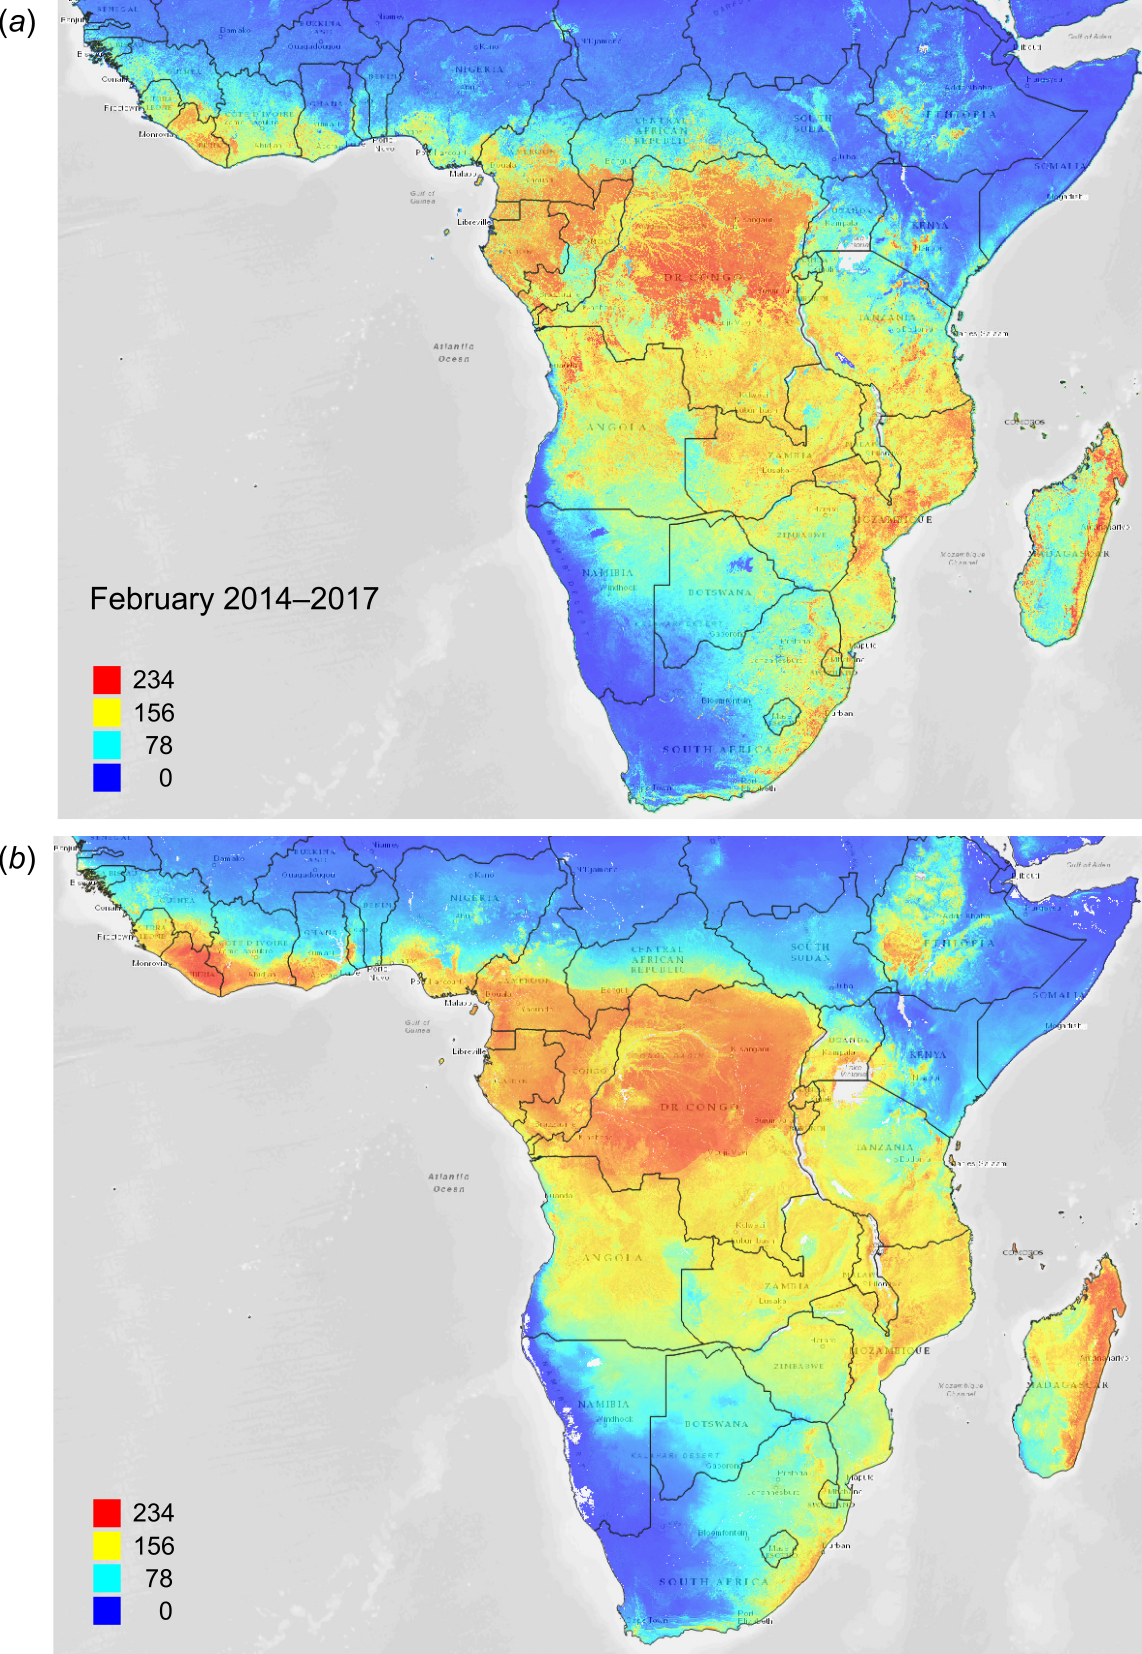
\includegraphics[width=.95\linewidth]{Fig_13.png}
\caption{FAPAR values for Subsaharan Africa: (a) actual (\SI{250}{\metre} resolution) and (b) predicted (\SI{1}{\kilo\metre} resolution) potential FAPAR values for February. Background map data: Google, DigitalGlobe.}
\label{Fig_actual_vs_potential_FAPAR_Feb_SSA}
\end{figure}

\begin{figure}[!hp]
\centering
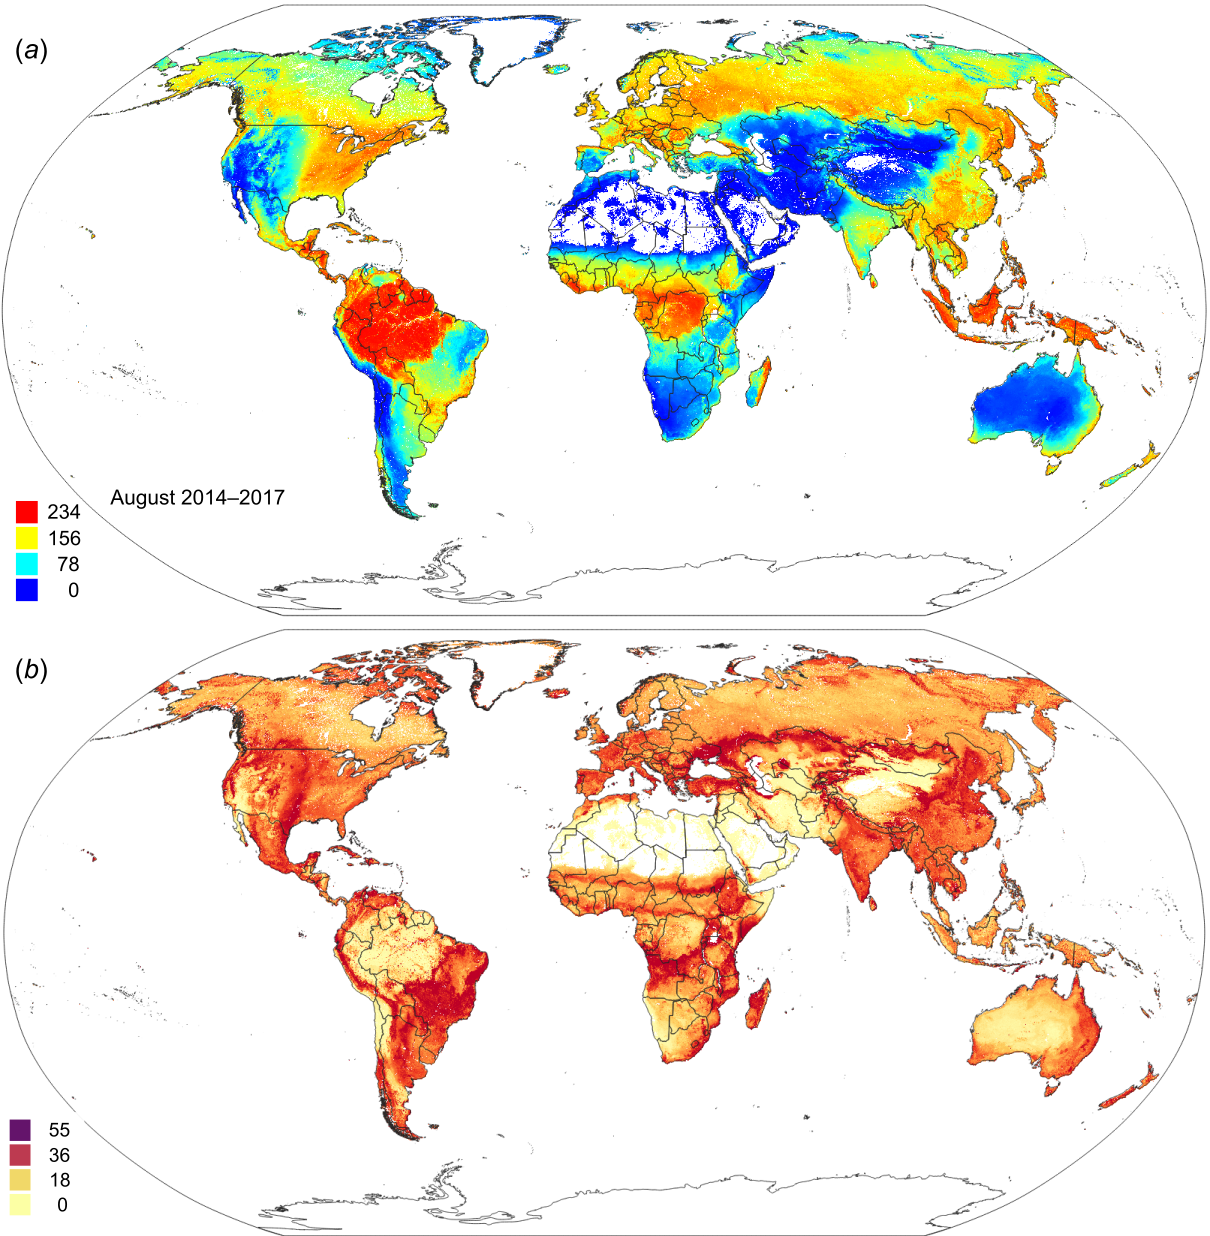
\includegraphics[width=\linewidth]{Fig_14.png}
\caption{Predicted global FAPAR values for August (a) and standard deviation of the prediction error for the map above (b). To convert to percent divide by 253.}
\label{Fig_FAPAR_predicted_global}
\end{figure}

Fig.\@~\ref{Fig_FAPAR_predicted_Sao_Paolo} depicts an example of actual vs predicted (PNV based) FAPAR for February in the urban area around S\~{a}o Paulo, where lower actual FAPAR reflects the removal of natural vegetation. Even larger differences between the potential and actual FAPAR are observed in parts of Africa (Fig.\@~\ref{Fig_actual_vs_potential_FAPAR_Feb_SSA}), likely reflecting land degradation and destruction of vegetation cover. In areas of intensive agricultural production (e.g.\@ Western Australia and Midwest USA), actual FAPAR can be much higher than potential FAPAR under potential natural vegetation in a given month. However this is often a temporal effect, as when PNV FAPAR is aggregated over the whole year, most places modified by human management show actual FAPAR is lower than potential. In Western Australian cropping zones for example, crop fields have higher FAPAR during the winter growing season, but since the fields are bare for most of the year, aggregated annual PNV FAPAR is higher overall. Whilst this pattern may hold for rain-fed agriculture, in intensively irrigated areas the FAPAR of the managed vegetation can be much higher than of the PNV over the whole year, especially in arid and semi-arid areas (e.g.\@ Nile Delta). This supplemental irrigation, plus the fact that total annual precipitation is the most important covariate, indicates that water availability/use efficiency is likely the main driver of FAPAR beyond natural conditions.  \par

Maps of the standard deviation (s.d.\@) of the prediction error (Fig.\@~\ref{Fig_FAPAR_predicted_global}) as derived in the \textsf{ranger} package by using the \verb"quantreg" setting \citep{meinshausen2006quantile} provide useful information about model quality i.e.\@ where collection of additional points would maximize model improvement and which additional covariates could be considered. For example, the highest prediction errors for FAPAR for the  month of August occurred in the transition areas between tropical forest and savanna areas, and in various biome transition zones in Asia. \par

\newpage
\section*{Discussion}

\subsection*{Accuracy and reliability of produced PNV maps}

Our results of modeling potential spatial distribution of global biomes, potential FAPAR and European forest tree taxa, show that relatively accurate maps of PNV can be produced using existing data and publicly available environmental grids. In the case of the biomes and forest tree taxa case studies, random forest consistently outperforms neural networks, gradient boosting and similar MLA's. This is consistent with some other vegetation mapping studies \citep{li2016comparison}. However, random forest and Cubist models perform equally well in the case of FAPAR. Accuracy assessment results of our work indicate improvement in product accuracy in terms of greater spatial detail and smaller classification error than found in the mapping products of \citet{levavasseur2012statistical} and \citet{tian2016terrestrial}. \par

Precipitation, temperature maps and bioclimatic images are consistently the most important covariates in all three case studies. Currently available lithology/parent material maps are not indicated as significantly important covariates in any of the case studies. This may be because the existing lithologic map \citep{GGGE:GGGE2352} is not detailed enough, and/or because the differences in lithology/parent material are more important at finer resolutions/scales than those mapped here. Landform and lithology/parent material covariates may be important at local scales but, globally, vegetation distribution seems to be dominated by climate. This is not surprising since nutrient availability is also partially controlled by climate and partially by the vegetation itself. Upon visualization of the mapping products however, it was noticed that the influence of topography is visible, especially in the maps of European forest tree taxa, suggesting that DEM derivatives are still important for mapping PNV.\par

We have also not considered any soil layers as inputs to modeling as these are also often predicted from similar climatic and remote sensing layers already used in our case studies as covariates. Moreover, most of the predictive soil mapping projects use RS images reflecting human induced changes, which we have tried to avoid as these are more relevant for mapping actual vegetation. For mapping of the Potential Managed Vegetation, however, it would be probably more important to include also soil property / soil type maps into the modeling framework.\par

Further improvements in prediction accuracy of global biome may be limited due to:

\begin{enumerate}
\item BIOME reconstructions representing the vegetation of an area around a given site rather than at the exact point location, since the source of the pollen is on the order of \@ 10--\SI{30}{\kilo\metre} around the site.
\item The ambiguity of reconstructions for about \SI{10}{\percent} of the sites, so that maximum accuracy of any prediction technique may not exceed \SI{90}{\percent} without additional observation data.
\item The fact that the BIOME reconstruction accuracy is known to be lower at ecotonal boundaries and in mountainous areas because of pollen transport issues, particularly the long-distance transport of tree pollen.
\item The BIOME data set is compiled from many regional reconstructions and all harmonization was done a posteriori, which may have introduced additional noise into the data.
\end{enumerate}
\par

So far, we did not explore opportunities for combining multiple MLA models based on validation data i.e.\@ for doing ensemble predictions, model averages or model stacks. Stacking models can improve upon individual best techniques, achieving improvements of up to $>$\SI{30}{\percent}, with the additional costs including higher computation loads \citep{michailidis2017investigating}. In our case, the extensive computational load from derivation of models and product predictions had already obtained improved accuracies, making increasing computing loads further a matter of diminishing returns.\par

Our list of MLA models could also be extended. For example, we did not consider the use of Support Vector Machines \citep{li2016comparison}, or the Extreme Learning Machine algorithm \citep{deo2015application}. Both have proven to be suitable for mapping vegetation distribution and quantitative properties of vegetation. Not all MLA methods are, however, suitable for large regression matrices, as the computing time can be excessive and hence parallelization options are crucial.\par 

Our models of PNV FAPAR are based on simulated point data and the accuracy of how well models represent natural vegetation areas is dependent on the representativeness of the \url{http://protectedplanet.net} and \url{http://intactforests.org} data. Also, many of the world's biomes such as the Mediterranean region and similar, have sustained high levels of human impact in the past and are perhaps under-represented in the \url{http://protectedplanet.net} data set. Nevertheless, our cross-validation results (Leave-Location-Out method) indicate a good match between training and validation points. \par

It would be useful to further explore what the performance of the models we used would be if we removed whole continents in the cross-validation process, or at least larger countries such as USA, China, Brazil, Australia, India and/or the South African Republic. For biomes, spatial Cross Validation showed a significant drop in accuracy; removing some larger countries from model training will likely also make difference. We did not explore effects of spatial proximity on mapping forest species and FAPAR as these are very dense point data sets. In addition, FAPAR training points were generated using simple random sampling, so spatial clustering should be non-existent.\par

\citet{fourcade2018paintings} recently demonstrated that randomly chosen classical paintings can also be added to predictive modeling, and sometimes such models might be even better evaluated than models computed using real environmental variables. MLAs have even higher tendency to over-fit data and often perform very poor in extrapolation areas. These two remain the biggest drawbacks of using MLAs for species distribution modeling. It appears that the key to avoiding over-fitting or using non-realistic mapping accuracy measures, based on \citet{fourcade2018paintings}, is in putting more effort in cross-validation (i.e.\@ making it more robust and more reliable) and in ensuring that most important predictors and partial correlations can also be explained.\par

\begin{figure}[!hbt]
\centering
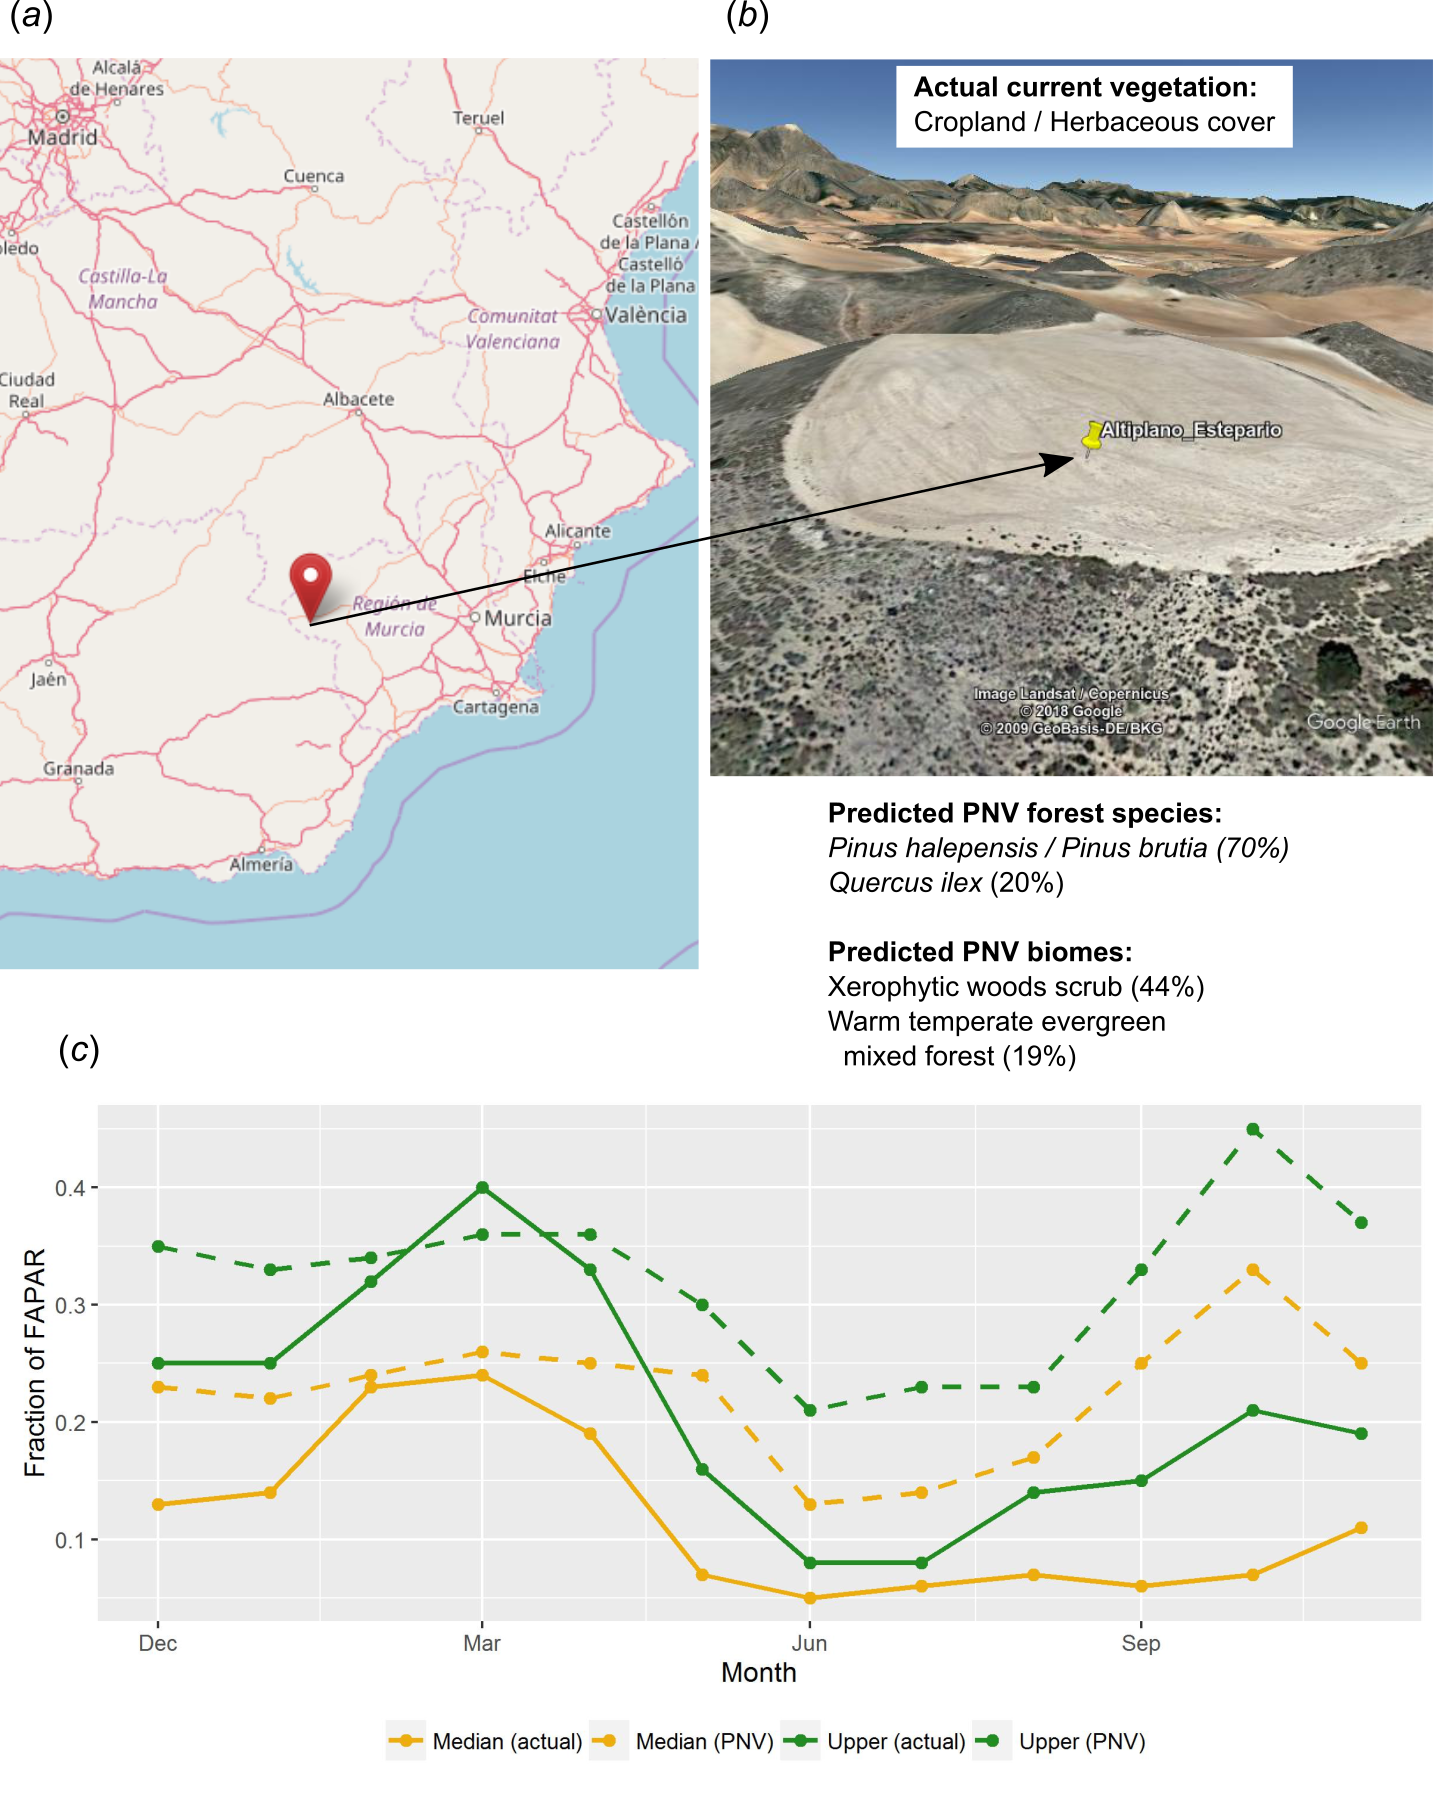
\includegraphics[width=\linewidth]{Fig_15.png}
\caption{Example of comparison between the actual land cover and actual FAPAR curves and our predicted potential natural vegetation (PNV) and predicted PNV FAPAR curves. According to our results, this location (a--b) in southern Spain (latitude=37.938478, longitude=-2.176692) currently utilizes \SI{51}{\percent} of the predicted FAPAR capability under PNV, indicating a substantive short fall in on-site photosynthetically active biomass (c). Background map (a) source: OpenStreetMap; landscape view (b) map data: Google, DigitalGlobe.}
\label{Fig_example_Altiplano_Estepario_assessment}
\end{figure}
%% TH: Correct coordinates: 37.937089,-2.1770248

\subsection*{Possible uses of the produced PNV maps}

\citet{newbold2016has} argued that many terrestrial biomes today have transgressed safe limits for biodiversity, with grasslands being most affected, and tundra and boreal forests least affected. \emph{``Slowing or reversing the global loss of local biodiversity will require preserving the remaining areas of natural (primary) vegetation and, so far as possible, restoring human-used lands to natural.''} \citep{newbold2016has} Roughly half of the difference of around 466 billion tonnes of carbon can be attributed to the clearing of forests and woodlands, mostly for agricultural purposes \citep{erb2017unexpectedly}. The other half of biomass carbon stock losses is derived from the management effects within a land cover class \citep{erb2017unexpectedly}. The expansion of agriculture will probably continue in the future, leading to decreased biodiversity and soil degradation \citep{mauser2015global,land6040067}. On the other hand, \citet{Griscom11645} identify reforestation (e.g.\@ biomass restoration) as the largest natural pathway to hold global warming below \SI{2}{\celsius}. In that context, accurate maps of PNV could become increasingly useful for assessing the level of land degradation/biomass shortfall relative to the potential of a site. Such information can also inform selection of optimal steps towards restoring biomass stocks in managed vegetation in ways that better reflect the PNV FAPAR in those areas. \par

Other uses of PNV maps include assessing the land potential i.e.\@ land use efficiency given the difference between actual and potential vegetation. Consider for example a location in southern Spain called \emph{``Altiplano Estepario''}, which has been identified by the Commonland company (\url{http://commonland.com}) and partners as a landscape restoration site. Fig.\@~\ref{Fig_example_Altiplano_Estepario_assessment} shows results of a spatial query for this location and values of our PNV and PNV FAPAR predictions, in comparison to the actual land cover and actual FAPAR images. The figure shows that the actual FAPAR is as good as PNV FAPAR in February and March but that differences are large in the summer months. Overall, the median and upper FAPAR for this specific location are only \SI{51}{\percent} of the PNV FAPAR, so we can say that this site is currently operating at \SI{51}{\percent} of the predicted FAPAR capability under PNV. This comparison should also consider that our estimates of FAPAR come with an RMSE of $\pm 0.085$. Furthermore, as landscape restoration efforts have recently begun on this site --- this work suggests that it ought to be possible to: (a) identify priority areas of PNV FAPAR shortfall, (b) use this information to inform in part the type of restoration strategies used, and (c) monitor the progress of restoration efforts in monthly time steps over several decades. Such practical measurement, monitoring and verification efforts are required to mobilize further investment in this emerging sector. \par

\begin{figure}[!hbt]
\centering
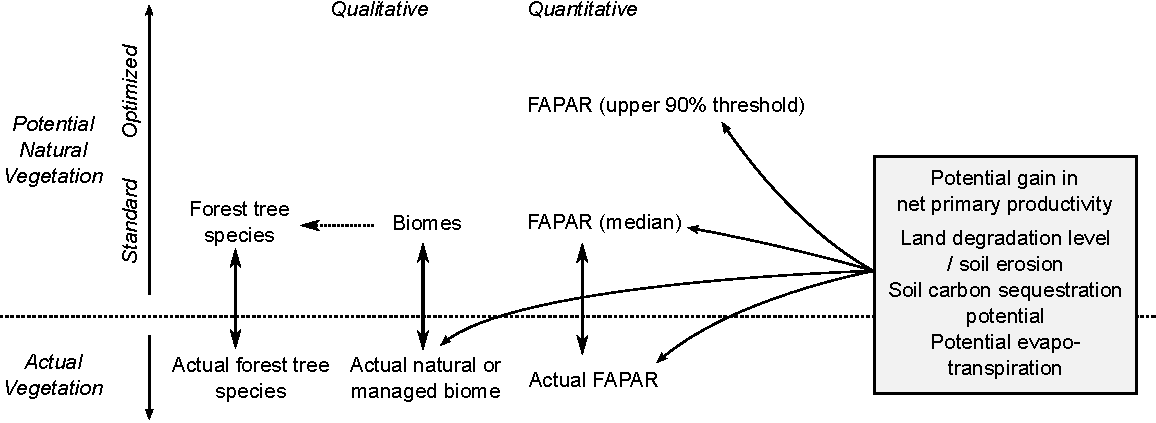
\includegraphics[width=\linewidth]{Fig_16.pdf}
\caption{Some possible uses of maps of Potential Natural Vegetation.}
\label{Fig_scheme_PNV_land_degradation_assessment}
\end{figure}

Our PNV maps could also be used to estimate soil carbon sequestration and/or evapotranspiration potential, and gains in net primary productivity assuming return of natural vegetation (Fig.\@~\ref{Fig_scheme_PNV_land_degradation_assessment}). Further more, by combining various estimates of potential natural and managed vegetation, one could design the optimal use of land both regionally and globally. \citet{herrick2013global}, for example, provide a theoretical framework for estimating land potential productivity which could theoretically connect all land owners in the world to share local and regional knowledge.\par

Maps of PNV for European tree species could also be used as a supplement to the distribution and ecology of tree species produced by \citet{san2016european} and \citet{brus2012statistical}. Species such as \emph{Carpinus orientalis}, \emph{Cupressus sempervirens}, \emph{Prunus mahaleb}, \emph{Sorbus domestica} are all predicted with TPR$<$0.5 indicating critically poor accuracy. Possible reasons for such low accuracy are problems with representation of training points and somewhat too broad ecological conditions, especially if a species follows some other more dominant tree species that have wide ecological niche. These maps should probably not be used for spatial planning.\par 

PNV for European tree species analysis could be made even more quantitative so that even predictions of dendrometric properties of tree species could be produced using similar frameworks. Also, similar PNV mapping algorithms could be used to map the potential canopy height based on the previously estimated map of the global canopy height \citep{Simard2011}.\par

\subsection*{Technical limitations and further challenges}

Running Machine Learning Algorithms on larger and larger data is computationally demanding; however, by using fully parallelized implementation of random forest in the \textsf{ranger} package, we were able to produce spatial predictions within days. Model fitting and prediction using EU Forest and GBIF data (1.5 million training points) was, however, very memory and time consuming and is not recommended for systems with $<$\SI{126}{\gibi\byte}~RAM. In our case, model fitting took several hours even with full parallelization, and  final models were $>$\SI{10}{\gibi\byte} in size. Prediction of probabilities took an additional 5--6 hours with the current computational set-up. In the future, scalable cloud computing could be used to overcome some of these computational limits. Machine learning will in any case continue to play a central role in analyzing large remote sensing data stacks and extracting useful spatial patterns \citep{LARY20163}.\par

With enough computing capacity, one could theoretically use all 160 million records of distribution of plant species currently available via GBIF \citep{Meyer2016EL} and from other national inventories to map global distribution of each forest tree species. In Europe the list is very short; globally this list could be quite long (e.g.\@ 60,000 species). The primary problems of using GBIF for PNV mapping will remain however, as these are primarily due to high clustering of points and under-representation of often inaccessible areas with very high biodiversity \citep{Yesson2007PLOS,Meyer2016EL}. GBIF records have been shown in the past to give biased results \citep{10.7717/peerj.2743}, so that spatial prediction methods that account for high spatial clustering, i.e.\@ bias in training point representation in both space and time; would need to be developed further to minimize such effects. \par

\section*{Conclusions}

Although PNV is a hypothetical concept, ground-truth observations can be used to cross-validate PNV models and produce an objective estimate of accuracy. As the prediction accuracy becomes more significant, the reliability of the PNV maps increases. Our analyses show that the highest accuracy for predicting 20 biome classes is about \SI{68}{\percent} (\SI{33}{\percent} with spatial Cross Validation) with the most important predictors being total annual precipitation, monthly temperatures and bioclimatic layers. Predictions of 73 forest tree species had a mapping accuracy of \SI{25}{\percent} and with average TPR of 0.69, with the most important predictors being mean annual and monthly temperatures, elevation and monthly cloud fraction. Regression models for FAPAR (monthly images) were most accurate with R-square of \SI{90}{\percent} (Leave-Location-Out CV) and with the most important predictors being total annual precipitation, MODIS cloud fraction images, CHELSA bioclimatic layers and month of the year, respectively. Machine learning can be successfully used to model vegetation distribution, and is especially applicable when the training data sets consist of a large number of observations and a large number of covariates. Extending the coverage of observations of natural and managed vegetation, including through making new ground observations, will allow regular improvements of such PNV maps. \par

\section*{Acknowledgments}
This research is a contribution to the AXA Chair Programme in Biosphere and Climate Impacts and the Imperial College initiative on Grand Challenges in Ecosystems and the Environment (ICP). Authors are grateful to \citet{karger2017climatologies} for maintaining the CHELSA Climate images, US agencies NASA and USGS for distributing high resolution images of Earth's atmosphere and the European Copernicus Land program. We are grateful to \citet{mauri2017eu} for sharing the EU-Forest --- a high-resolution tree occurrence dataset for Europe. We are also grateful to the Open Source software developers of the packages \textsf{ranger}, \textsf{xgboost}, \textsf{caret}, \textsf{raster}, \textsf{GDAL}, \textsf{SAGA GIS} and similar, and without which this work would have not be possible.

\bibliography{PeerJ_27103}

\end{document}